
	\section{Materiales y Métodos}
	\label{seccion:Cuatro}
		La presente sección describe en detalle los procedimientos, herramientas y metodologías empleadas en el diseño, desarrollo y evaluación del sistema Torddis. Este sistema combina tecnologías avanzadas de Internet de las Cosas (IoT) e Inteligencia Artificial (IA) para monitorizar y mejorar la concentración de los estudiantes en actividades académicas realizadas en el hogar. El enfoque metodológico estuvo guiado por la metodología TDDM4IoTS, permitiendo un desarrollo iterativo y enfocado en la calidad técnica y pedagógica.
		
		A través de este apartado, se exponen las características de los participantes, el diseño experimental, las técnicas utilizadas para la validación de instrumentos y análisis de datos, así como los aspectos técnicos del sistema. Además, se destacan las medidas adoptadas para reducir sesgos, asegurar la confiabilidad de los resultados y responder a las necesidades educativas y tecnológicas de los usuarios finales. Finalmente, se reconocen las limitaciones del estudio y se justifica el impacto pedagógico del sistema en el desarrollo de habilidades de autorregulación y aprendizaje autónomo.
		
		\subsection{Participantes y Contexto del Estudio}
			El estudio incluyó la participación de 12 niños con su respectivo tutor, seleccionados mediante un muestreo por conveniencia. Los niños tenían edades comprendidas entre los 7 y 12 años, cursando estudios primarios y secundarios. Los tutores, de entre 25 y 65 años, presentaban niveles de educación primaria y secundaria. Los participantes residen en sectores urbanos y rurales con servicios básicos (electricidad, agua potable, Internet y telefonía móvil).
			
			El criterio de selección garantizó que los hogares contaran con acceso a Internet en el domicilio (WiFi o datos móviles) y datos móviles en el Smartphone del tutor, condiciones necesarias para implementar el sistema. Este enfoque asegura que los participantes representan el perfil de los usuarios potenciales de Torddis: familias con tutores ocupados en actividades dentro y fuera del hogar, responsables de niños en edad escolar que necesitan supervisión directa.
			
			La representatividad de la muestra se considera aceptable al trabajar con usuarios reales del sistema y cumplir con criterios de inclusión definidos. La selección por conveniencia es adecuada en investigaciones preliminares como esta, permitiendo obtener una muestra significativa pese a la limitada disposición de colaboración de algunas familias \citep{DiPietro2025Meta}.
		
		\subsection{Proceso Experimental y Validación de Instrumentos}
			El proceso experimental se llevó a cabo en dos etapas:
		
			\subsubsection{Entorno simulado}
				Diseñado para evaluar la usabilidad y rendimiento del sistema. Durante esta fase, los tutores usaron Torddis durante 30 minutos en un entorno controlado, donde se verificaron todas las funcionalidades del sistema. Se emplearon cuestionarios SUS y preguntas abiertas para recopilar datos sobre la experiencia del usuario.
			
			\subsubsection{Entorno real}
				Diseñado para evaluar la efectividad del sistema. Esta fase duró una semana, considerando que solo existía un prototipo. Se utilizó un cuestionario con escala de Likert para medir la percepción de los tutores sobre la utilidad y efectividad de Torddis (ver \ref{Appendix:Effectivity}), incluyendo preguntas sobre atracción del dispositivo, precisión de las notificaciones, y su impacto en la autorregulación y concentración de los niños \citep{Ackermans2025Young}.
			
				La validez de los instrumentos fue garantizada mediante la revisión y validación por investigadores con experiencia, quienes aseguraron la claridad de las preguntas y su adecuación al propósito del estudio. Además, los datos generados por el sistema (e.g., detección de objetos, alertas) fueron corroborados manualmente para garantizar su precisión \citep{Wang2025Development}. Además, se analizó si las variables siguen una distribución normal o no para, según el tipo de variable calcular los estadísticos para determinar la diferencias (ANOVA, Kruskal-Wallis), y coeficientes de correlación entre las variables (Pearson y Spearman).
		
		\subsection{Aleatorización y Sesgos}
			No se implementó un proceso de aleatorización debido a la naturaleza del muestreo por conveniencia. Sin embargo, se tomaron medidas para minimizar sesgos, como \citep{Huang2025How}:
			
			\begin{itemize}
				\item Explicación detallada de las preguntas del cuestionario antes de su llenado.
				\item Garantía de anonimato y confidencialidad de las respuestas.
				\item Aplicación del cuestionario sin la presencia de los investigadores para evitar influencia en las respuestas.
			\end{itemize}
		
			Reconocemos que podrían existir sesgos relacionados con la cercanía de los investigadores a los participantes, lo que podría influir en las respuestas de los cuestionarios \citep{DiPietro2025Meta}.
		
		\subsection{Análisis Estadístico}
			Los datos obtenidos fueron analizados utilizando métodos descriptivos y correlacionales. Para las evaluaciones de usabilidad (SUS), se calculó un puntaje promedio para determinar la aceptación del sistema. En la fase real, se empleó análisis correlacional para explorar relaciones entre las variables medidas (e.g., percepción del tutor sobre la mejora en la autorregulación y concentración de los niños) \citep{Wang2025Development}.
		
			El análisis estadístico permite identificar patrones significativos en el uso del sistema, justificando su validez en contextos similares. Los métodos empleados son apropiados para estudios piloto, donde el tamaño de la muestra limita el uso de pruebas inferenciales más robustas.
		
		\subsection{Desarrollo de TORDDIS}
			El desarrollo del sistema Torddis siguió una metodología estructurada para asegurar la integración efectiva de los componentes de hardware y software, con el objetivo de proporcionar una herramienta integral para monitorizar y mejorar la concentración de los estudiantes en casa. Esta sección detalla los materiales y métodos utilizados en el diseño, desarrollo y evaluación del sistema Torddis.
			
			Más específicamente, Torddis se desarrolló utilizando la metodología TDDM4IoTS \citep{Guerrero-Ulloa2020TDDM4IoTS}. Esta metodología es la más completa respecto al ciclo de vida del sistema \citep{Guerrero-Ulloa2023Review} y ha sido ampliamente valorada \citep{Guerrero-Ulloa2023DevIdeAir,Guerrero-Ulloa2023IdeAir,Guerrero-Ulloa2023SP4,Guerrero-Ulloa2023Nawi}. Durante el desarrollo del proyecto tecnológico, se implementaron todas las etapas de la metodología, excepto la última, mantenimiento, debido al corto tiempo de vida del sistema al momento de la redacción de este artículo. Además, este marco metodológico ayuda en la detección temprana de errores, contribuyendo a reducir los costos y el tiempo de desarrollo, permitiendo un código más limpio \citep{Beck2002TDD}.
			
			El equipo de proyecto estuvo compuesto por los autores del trabajo, con los roles de los miembros del equipo detallados en la Tabla \ref{tab:Roles}.
			
			\begin{table}[H]
				\caption{Roles desempeñados por los miembros del equipo.\label{tab:Roles}}
				\begin{tabularx}{0.8\textwidth}{>{\arraybackslash}X >{\arraybackslash}X}
					\toprule
					\textbf{Rol}	& \textbf{Miembro}\\
					\midrule
					Cliente/Usuario final & Autor 5, Autor 6 y algunos padres\\
					Facilitador del proyecto		&  Autor 1 y Autor 4\\
					Equipo de desarrollo		&  Autor 2 y Autor 3\\
					Consejero		&  Alternando entre Autor 2 y Autor 3\\
					\bottomrule
				\end{tabularx}
			\end{table}
			
			\subsubsection{Análisis Preliminar}
				Esta etapa fue una etapa crucial, ya que se pudo determinar si el proyecto era viable para su desarrollo o no. Para determinar su viabilidad se desarrollaron algunas actividades.
			
				\subsubsection*{Análisis de Requisitos Preliminares}
					Este análisis de los requisitos preliminares abarcó tanto los aspectos funcionales (especificaciones del cliente) como los no funcionales (atributos de calidad del sistema) a un nivel general de detalle.
					
					El equipo de proyecto logró reclutar a un usuario tutor con una necesidad inminente de un sistema como Torddis, permitiendo un rápido análisis preliminar de sus necesidades. Además, se reclutó a un grupo de usuarios tutores para verificar los requisitos propuestos en esta actividad. Posteriormente, todos estos actores¡, apoyaron para realizar el análisis detallado de los requisitos del sistema.
					
					En esta actividad se determinó que los requisitos funcionales que Torddis debe cumplir son \citep{Asish2022Detecting,Pabba2022AnIntelligent,Vettivel2018System}:%Yin2021}:
					
					\begin{itemize}
						\item Registrar y modificar los datos del usuario tutor.
						\item Permitir al usuario tutor registrar y modificar los datos del niño en la aplicación móvil.
						\item Permitir al usuario tutor habilitar y/o deshabilitar los objetos que están permitidos en el área de estudio (escritorio).
						\item Monitorizar la presencia del niño, las expresiones faciales, el estado de somnolencia y el uso de los objetos que no están permitidos en el área de estudio (escritorio).
						\item Visualizar el historial del monitorización de los parámetros de distracción del niño.
						\item Reproducir un sonido de alarma y luz led mientras el niño se aleje del área de estudio (escritorio) o tenga signos de soñolencia.
						\item Generar gráficos estadísticos sobre los eventos sucedidos: ha estado con sueño, ha usado objetos restringidos y el conteo de cada expresión facial del niño de los últimos 7 días a partir de una fecha seleccionada.
					\end{itemize}
					
					Los requisitos no funcionales que debe cumplir el sistema propuesto son:
					
					\begin{itemize}
						\item La aplicación móvil de tener una interfaz minimalista e intuitiva.
						\item El dispositivo debe tener dimensiones como de algo cotidiano para el niño (juguete).
						\item Al ser un dispositivo para estar en un lugar determinado (lugar destinado para hacer tareas escolares), debe ser alimentado por el sistema de electricidad público.
						\item Los datos personales y de autenticación deben ser encriptados para asegurar la privacidad de los datos.
						\item Utilizar la red WiFi disponible en el hogar.
					\end{itemize}
					
					Para el análisis de los requisitos se utilizaron diagramas de casos de uso, empleando la herramienta web gratuita TDDT4IoTS disponible en \href{https://aplicaciones.uteq.edu.ec}{https://aplicaciones.uteq.edu.ec} o \href{http://www.tddt4iots.com}{http://www.tddt4iots.com}. 
					
					Además, se determinaron las tecnologías a utilizar para el desarrollo de Torddis, incluyendo recursos de hardware, tecnologías y herramientas de software para el desarrollo de la aplicación móvil y la configuración del hardware. La elección de los recursos se basó en los criterios de selección de los autores, como el uso de herramientas y tecnologías de software de código abierto con documentación adecuada y suficiente que cumplan con las funcionalidades requeridas y que el equipo de desarrollo tenga la experiencia necesaria.
					
					Entre las tecnologías de inteligencia artificial que se consideraron para su selección están los métodos para:
					
					\begin{itemize}
						\item Reconocimiento Facial
						\item Reconocimiento de Expresiones Faciales
						\item Detección de Sueño
						\item Reconocimiento de Objetos
						\item Monitorización de las Distracciones de los Niños, según los parámetros de distracción
					\end{itemize} 
					Asimismo, para el hardware IoT se consideró importante que cumpla con las funcionalidades requeridas, sea económico, esté disponible en el mercado local, y cuente con la documentación necesaria para su implementación. También se valoró que el equipo de desarrollo tuviera experiencia en su configuración y uso.
					
					Estas tecnologías permiten ajustar las estrategias de monitoreo en tiempo real según las necesidades detectadas en el comportamiento de los estudiantes, maximizando la eficacia del sistema al proporcionar una supervisión personalizada. Investigaciones recientes han destacado que herramientas basadas en inteligencia artificial, como ChatGPT, no solo pueden generar contenido educativo adaptado, sino también ofrecer retroalimentación personalizada. Este enfoque subraya el potencial de la IA para optimizar los procesos educativos y fomentar entornos de aprendizaje más centrados en el estudiante, donde la personalización y la supervisión se integran de manera efectiva \citep{Wang2025Development, Li2024Systematic}.
				
				\subsubsection*{Análisis de viabilidad}
					Este análisis se realizó desde los tres aspectos considerados en la metodología TDDM4IoTS: viabilidades técnica, económica y operativa. La disponibilidad de los recursos de hardware y software necesarios para el desarrollo de Torddis fue crucial para garantizar el éxito de este proyecto. Además, la presencia de un equipo de desarrollo con las habilidades y conocimientos adecuados permitió completar Torddis con un presupuesto muy limitado y con un cronograma reducido.
				
				\subsubsection*{Viabilidad Técnica}
					Se analizaron las tecnologías disponibles para el desarrollo de Torddis, incluyendo recursos de hardware, algoritmos y métodos de IA, y herramientas de software para monitorizar las distracciones de los estudiantes durante sus actividades escolares.
				
					Siempre buscando responder a las preguntas de investigación planteadas en este documento, se realizó una revisión acerca de las tecnologías de software, IA y hardware y otros recursos existentes y su aplicación en entornos educativos ayudó a seleccionar las tecnologías más apropiadas para este proyecto.
					
					Para la selección de los componentes de hardware se aplicaron los siguientes criterios:
					
					\begin{enumerate}
						\item \textbf{Disponibilidad:} El componente debía estar disponible en la tienda. Dado que no existe un mercado directo en el lugar de residencia del facilitador de proyecto para adquirirlo, se buscaron tiendas en línea (www.mercadolibre.com.ec). La tienda debía ser confiable. 
						\item \textbf{Tiempo de entrega:} Dentro de la disponibilidad también se consideró el tiempo de entrega. Este plazo no debía superar las 48 horas.
						\item \textbf{Precio:} El componente a adquirir debe ser económico. Es decir, la tienda seleccionada debe ser entre las confiables la que lo oferte a menor precio.
						\item \textbf{Documentación:} La disponibilidad de documentación en línea para el uso adecuado del componente seleccionado.
						\item \textbf{Experiencia:} El equipo de desarrollo debe tener experiencia en la configuración del componente.
					\end{enumerate}
				
					Así mismo, el cronograma de actividades para el desarrollo del prototipo de TORDDIS estuvo dentro del periodo de tiempo adecuado.
				
				\subsubsection*{Viabilidad Financiera}
					En cuanto a lo financiero, el prototipo de TORDDIS se considera muy económico. Fue desarrollado utilizando herramientas, y tecnologías de Software e inteligencia artificial gratuitas. Los recursos financieros fueron dirigidos exclusivamente para obtener los componentes de hardware necesarios.
				
				\subsubsection*{Vialidad Operativa}
					Al considerar los requisitos no funcionales de TORDDIS, se garantiza que los usuarios tutores puedan manipular el dispositivo y manejar la aplicación móvil a su conveniencia. Por lo tanto la viabilidad operativa, se garantiza. Además estos mismos requisitos garantizan el cumplimiento de la garantía de la privacidad de los datos personales.
			
			\subsubsection{Diseño de la Capa Tecnológica}
				Uno de los objetivos conseguidos en esta fase es el diseño de la arquitectura del sistema. La arquitectura es una guía importante para que los desarrolladores logren su objetivo con calidad \citep{Liu2011Status}. Para ayudar a los tutores que tienen múltiples ocupaciones sean dentro o fuera del hogar, se consideró la construcción de un dispositivo IoT para determinar el estado del niño mientras hace tareas escolares. 
			
				Para el diseño de la arquitectura de TORDDIS, se consideró: Siendo que el tutor no puede estar presente todo el tiempo al lado de su representado ¿Cómo suplir la presencia del tutor para vigilar al estudiante mientras realiza sus tareas escolares en su hogar?
			
				Si el tutor se encuentra fuera del hogar, ¿Cómo informarlo de los eventos sucedidos con su tutorado?, ¿Cómo el tutor persuade al estudiante para que continúe haciendo sus tareas escolares? 
			
				El análisis de estás interrogantes fue crucial para diseñar un sistema que ayude a los tutores a apoyar el aprendizaje de sus tutorados y mejorar su rendimiento académico, incluso mejorar su concentración mientras realizan sus tareas escolares.
			
			\subsubsection{Análisis detallado de requisitos}
				El análisis de requisitos fue una primera fase que se desarrollo de manera iterativa, es decir para cada uno de los entregables. Los dos entregables fueron el dispositivo y la aplicación móvil. Así mismo cada uno de los componentes en los que se dividió cada uno de los entregables, a su vez se ejecutaron por tareas. Estas tareas tuvieron una duración de dos hasta seis semanas inclusive (por la disponibilidad de tiempo).
			
				Los componentes al ser desarrollados uno por uno, el posterior fue integrado con el/los anterior/es. Por lo tanto, al terminar el último componente, el entregable estaba listo para ser usado y probado.
			
				El detalle de los requisitos se consideró primeramente lo encontrado en la literatura, y se tomó decisivamente lo que los futuros usuarios especificaron. Esto se detalló en un formato de casos de uso semiestructurados para guardar un estándar enmarcado en una estructura definida previamente \citep{Zegzhda2018Use}.
			
			\subsubsection{Generación y Refinamiento del Modelo}
				Cómo TDDM4IoTS \citep{Guerrero-Ulloa2020TDDM4IoTS} sugiere que no todas las etapas deben ser ejecutadas y que el orden puede variar, la etapa de refinamiento de modelos no se ejecutó.
			
				Esta etapa de refinamiento de modelos, los desarrolladores consideran que es importante cuando los requisitos no están claros al inicio del desarrollo y se vuelven más específicos a medida que avanza el ciclo de vida del proyecto. Caso que no sucedió en el desarrollo de TORDDIS, los requisitos fueron claros desde el inicio.
			
				Además, la no ejecución de esa etapa la atribuyen a la herramienta usada \citep{Guerrero2024Test}, en vista de qué, el refinamiento del modelo se hace dentro de los casos de uso, y ella se encarga de actualizar los modelos. El modelo al ser obtenido directamente de las especificaciones de los casos de uso, y TORDDIS al no tener una envergadura que demanda un esfuerzo extraordinario para su modelado, el modelo obtenido usando TDDT4IoTS fue el ideal.
			
			\subsubsection{Generación de Pruebas}
				Las pruebas necesarias en el desarrollo de TORDDIS fueron las pruebas unitarias, las pruebas de integración, las pruebas de sistemas y las pruebas de aceptación \citep{Sciarra2024Smash}.
			
				\begin{itemize}
					\item Las \textit{pruebas unitarias} son las más extensas pero simples que sirvieron para que los desarrolladores ahorren tiempo en la detección y corrección de errores \citep{Mafi2024Regression}
					\item Las pruebas de integración fueron ejecutadas para integrar cada uno de los componentes de los entregables, y a su vez en para verificar que las partes que interactúan lo hagan correctamente, por ejemplo los servicios web con la la base de datos, y en su momento, estos con la lógica de negocios de la aplicación móvil, garantizando así que el sistema cumpla con los requisitos especificados por los usuarios.
					\item Las pruebas de sistema se ejecutaron para integrar los entregables en un sistema. Es decir ya las partes más grandes del sistema.
					\item Después que el equipo de desarrollo probó todo el sistemas, el usuario ejecutó las pruebas de de aceptación. Para el equipo del proyecto, las pruebas de aceptación sirvieron para evaluar el sistema por parte de los usuarios.
				\end{itemize}
			
			\subsubsection{Generación y Refinamiento del Software} 
				El desarrollo del software para el sistema Torddis se llevó a cabo en dos etapas principales: generación y refinamiento. Inicialmente, el código fue escrito tomando como base los modelos y pruebas generados automáticamente por la herramienta TDDT4IoTS \citep{Guerrero2024Test}, complementado por los desarrolladores para los aspectos no automatizados. 
			
				Durante esta etapa, se verificaron todos los componentes de software mediante la ejecución de las pruebas diseñadas para garantizar su funcionalidad y su alineación con los requisitos establecidos.
			
				Posteriormente, en la etapa de refinamiento, el software fue mejorado para optimizar su calidad y rendimiento. Los cambios realizados incluyeron la reducción de variables temporales o auxiliares para una aplicación de la computación verde \citep{Firmansyah2024Integrating}, el mejoramiento del nombrado de atributos, métodos y clases para facilitar la comprensión del código, y la adición de comentarios en las partes más importantes del mismo. Estas mejoras contribuyeron a un código limpio, mantenible y de mayor calidad, fortaleciendo la solidez del sistema Torddis en su conjunto \citep{Marabesi2024Exploring}.
			
			\subsubsection{Despliegue de Hardware y Software}
				Cada uno de los componentes de los entregables fue desplegado en el medio que finalmente fue desplegado todo el entregable en condiciones de despliegue del sistema en su conjunto. Los componentes de la aplicación móvil eran probados en el simulador de Android Studio, y luego de ser generado el apk iterativa, esa aplicación móvil se desplegó en un smartphone con las características mínimas para las cuales fue desarrollada.
			
				El despliegue de los componentes del entregable final o del dispositivo Torddis se desplegaron iterativamente en ambientes simulados o de pruebas en pleno desarrollo. Posteriormente, el para hacer las pruebas de integración y de sistema se desplegó en un entorno real-ideal, donde cualquier estudiante escolar puede realizar tareas escolares.
			
			\subsubsection{Evaluación de los Entregables}
				Durante el desarrollo del proyecto y para evaluar la funcionalidad y usabilidad de Torddis. Se consideraron las capacidades de los usuarios tutores para garantizar que Torddis permaneciera operativo después de su implementación, sin la necesidad de personal adicional, excepto en casos de mantenimiento correctivo, donde personas con conocimientos sobre el desarrollo de Torddis tendrían que intervenir.
			
				Para la evaluación de la usabilidad se utilizó un formato para obtener el consentimiento informado (ver anexo \ref{Appendix:InformedConsent}), luego una encuesta demográfica (ver anexo \ref{Appendix:DemographicSurvey}) para conocer el contexto de los evaluadores, un cuestionario SUS con dos grupos de preguntas, uno con escala de Likert (ver anexo \ref{Appendix:LikertScale}) y otro de preguntas abiertas (ver anexo \ref{Appendix:OpenQuestions}).
			
			\subsubsection{Mantenimiento}		
				La planificación del mantenimiento debe basarse en el tiempo de vida útil de los componentes del dispositivo, complementándose con mantenimientos preventivos realizados trimestralmente. Es esencial asegurar un entorno adecuado para su uso, prestando especial atención a la limpieza y reduciendo al máximo la presencia de polvo, humedad y la exposición directa a la luz solar.
				
				La frecuencia de los mantenimientos preventivos debe alinearse con la vida útil promedio del componente con menor durabilidad. Además, se recomienda disponer de repuestos para dichos componentes y mantener una copia actualizada del software utilizado para configurar el hardware IoT.
				
				El mantenimiento de la aplicación móvil debe realizarse, como mínimo, una vez al mes. Este procedimiento es necesario para gestionar el aumento de datos almacenados, lo que podría derivar en un uso innecesario de recursos. En caso de requerirse cambios en la lógica de negocios o en los requisitos del usuario, como modificaciones en los reportes, será indispensable contar con un ingeniero de software que pueda implementar dichas actualizaciones de forma adecuada.
				
		\subsection{Limitaciones y Generalización}
			El estudio presenta ciertas limitaciones:
			
			\begin{enumerate}
				\item La muestra se limita a un grupo pequeño de participantes seleccionados por conveniencia, lo que podría no representar otros contextos sociodemográficos o tecnológicos.
				\item La duración de la fase real (una semana) no permite evaluar el impacto a largo plazo del sistema en habilidades como la autorregulación.
				\item La disponibilidad de un único prototipo restringió la simultaneidad del uso por varios participantes.
			\end{enumerate}
			
			Estas limitaciones son comunes en investigaciones que exploran el impacto de tecnologías educativas en contextos iniciales o pilotos \citep{Gregg2021Promissing,Jonsson2004Appropriating}. Estudios previos han destacado que la generalización de los resultados en intervenciones tecnológicas depende en gran medida de las características específicas de la población y del entorno en el que se implementan \citep{Song2013Development}. Por ejemplo, una meta-análisis reciente sobre los efectos de la tecnología en estudiantes desfavorecidos resalta cómo las variaciones en el acceso a recursos y las condiciones contextuales pueden influir significativamente en los resultados obtenidos, sugiriendo la necesidad de diseñar futuros estudios que incluyan una muestra más amplia y diversa para aumentar la representatividad de los hallazgos \citep{DiPietro2025Meta}.
			
		\subsection{Validación de la Metodología TDDM4IoTS}
			La metodología TDDM4IoTS \citep{Guerrero-Ulloa2020TDDM4IoTS} fue seleccionada por su enfoque en proyectos IoT, permitiendo la integración iterativa de hardware y software. Durante el desarrollo de Torddis, esta metodología facilitó:
			
			\begin{itemize}
				\item La definición de requisitos funcionales y no funcionales, basada en las necesidades de los tutores.
				\item La generación automática de pruebas, reduciendo tiempos y errores en el desarrollo.
				\item La validación temprana de componentes, asegurando la robustez del sistema.
			\end{itemize}
			En comparación con metodologías tradicionales, TDDM4IoTS destaca por su capacidad de adaptarse a proyectos con múltiples entregables interdependientes, como los que combinan IoT y aplicaciones móviles. Además, es la metodología que garantiza el cumplimiento del ciclo de vida de los sistemas \citep{Guerrero2023Agile,ISO-IEC-IEEE12207-2017,ISO-IEC-IEEE12207-2017Application}.
			
			Metodologías estructuradas como TDDM4IoTS son particularmente efectivas en el desarrollo de sistemas educativos basados en tecnología, ya que permiten integrar de manera eficiente componentes tecnológicos y pedagógicos. Según investigaciones recientes sobre sistemas de aprendizaje adaptativo, la aplicación de enfoques metodológicos claros no solo asegura un desarrollo robusto, sino que también optimiza la alineación entre las funcionalidades del sistema y las necesidades específicas de los usuarios finales. Este enfoque metodológico es clave para abordar los desafíos de interoperabilidad y personalización en contextos educativos \citep{Wang2025Development}.
			
		\subsection{Justificación Pedagógica}
			El diseño del sistema y la metodología aplicada están alineados con objetivos pedagógicos clave, como fomentar habilidades de autorregulación y aprendizaje autónomo en los estudiantes. A través de retroalimentación inmediata y personalización, Torddis ayuda a los estudiantes a gestionar su atención y tiempo, mientras que los tutores pueden supervisar y apoyar el proceso de aprendizaje \citep{Chen2025Unpacking}.
			
			Además, las etapas iterativas del desarrollo, guiadas por TDDM4IoTS, permitieron incorporar mejoras pedagógicas en cada fase, asegurando que el sistema responda tanto a necesidades tecnológicas como educativas \citep{Huang2025How}.
			
	\section{Resultados y Discusión}
	\label{seccion:Cinco}
		A continuación se presentan los resultados de cada una de las fases de desarrollo del sistemas según la metodología aplicada. Así como, los hallazgos obtenidos a través de diversas evaluaciones realizadas al prototipo del sistema Torddis. Estas evaluaciones incluyen pruebas funcionales, cuestionarios de usabilidad y análisis de datos demográficos y de monitorización, con el objetivo de determinar la efectividad y aceptación del sistema desde una perspectiva tanto técnica como de experiencia del usuario.
		
		Los resultados obtenidos se detallan a continuación, proporcionando una visión integral del rendimiento y utilidad del sistema Torddis en su contexto de aplicación.
		
		\subsection{Desarrollo del Sistema Prototipo TORDDIS}
			Los resultados de cada una de las etapas de la metodología TDDM4IoTS \citep{Guerrero-Ulloa2020TDDM4IoTS} se exponen en cada una de los siguientes apartados.
			
			\subsubsection{Análisis Preliminar}
				El análisis a grano grueso de los requisitos funcionales se muestran en el diagrama general de casos de uso que se muestra en la Figura \ref{fig:UseCaseDiagram}). Estas funcionalidades y sus responsables fueron consideradas con base a las entrevistas iniciales con el usuario final y los educadores.
				
				El usuario \textit{tutor} es la persona encargada de configurar los \textit{objetos permitidos}, \textit{monitorizar} a sus \textit{estudiantes}, recibir las alertas emitidas por el sistema por los eventos sucedidos, y persuadir a su estudiante monitoreado. Además, el usuario tutor puede visualizar los informes y los eventos históricos.
				
				\begin{figure}[h]
					\centering
					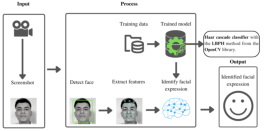
\includegraphics[frame,scale=0.5, width=\linewidth]{figs/Figure_2}
					\caption{Modelado de los requisitos del usuario a un nivel alto.\label{fig:UseCaseDiagram}}
				\end{figure} 
				
				\subsubsection*{Recursos de Hardware}
					La Tabla \ref{table:hardware-components} describe los recursos de hardware IoT utilizados para construir Torddis. 
					
					\begin{table}[htb]
						\caption{Componentes de hardware.}
						\label{table:hardware-components}
						\centering
						\begin{tabular}{p{0.23\textwidth}p{0.15\textwidth}p{0.15\textwidth}p{0.35\textwidth}}
							\hline
							\multicolumn{1}{l}{\textbf{Funcionalidad}} & \multicolumn{1}{l}{\textbf{Seleccionado}} & \multicolumn{1}{l}{\textbf{Alternativas}} & \multicolumn{1}{l}{\textbf{Observación}} \\ \hline
							Conectividad con el servicio web y transmisión de video & Esp32cam & Cámara Ov7670 VGA & Este módulo tiene conectividad WiFi + Bluetooth y una cámara de video integrada \citep{CasasSanchez2022}. \\
							Transmisión de información & Esp8266 NodeMcu v3 & Arduino UNO, Módulo GSM & El módulo NodeMCU es una pequeña placa que proporciona conexión WiFi para la transmisión de datos al servicio web \citep{Barai2019}. \\
							Sonido de alarma & Zumbador pasivo & Zumbador activo & Comúnmente utilizado para generar alarmas sonoras en placas electrónicas \citep{Adebisi2023development}. \\
							Emisor de luz para alerta & LED de 5mm (cualquier color) & LED RGB & Diodo LED transparente brillante utilizado para configurar una alarma \citep{Upender2020}.  \\ \hline
						\end{tabular}
					\end{table}
				
				\subsubsection*{Tecnologías de Software}
					El desarrollo del sistema propuesto requirió el uso de diversas tecnologías, que abarcan lenguajes de programación y algoritmos de IA, para apoyar eficazmente el logro de los objetivos planteados. La Tabla \ref{table:software-technologies} presenta las tecnologías de software utilizadas en la construcción del sistema Torddis.
				
					\begin{table}[hbt]
						\caption{Tecnologías de software utilizadas en la construcción del sistema Torddis.}
						\label{table:software-technologies}
						\centering
						\begin{tabular}{p{0.23\textwidth}p{0.15\textwidth}p{0.15\textwidth}p{0.35\textwidth}}
							\hline
							\multicolumn{1}{l}{\textbf{Funcionalidad}} & \multicolumn{1}{l}{\textbf{Alternativas }} & \multicolumn{1}{l}{\textbf{Seleccionado}} & \multicolumn{1}{l}{\textbf{Observación}} \\ \hline
							Aplicaciones móviles para Android & Kotlin & Java & Lenguaje utilizado en Android Studio con una gran comunidad en el campo del desarrollo de aplicaciones móviles \citep{Sharma2021Real-Time}. \\
							Aplicaciones de IA & Java, R & Python & Lenguaje de programación con bibliotecas de código abierto populares para el desarrollo de aplicaciones de IA \citep{Cai2005OnThePerformance}. \\
							Aplicaciones y servicios web & Flask & Django & Marco popular con capacidades de desarrollo rápido y previene errores de seguridad en el desarrollo de aplicaciones o servicios web \citep{Puneet2022ADjango}. \\
							Bases de datos & MySQL, Microsoft SQL Server & PostgreSQL & Base de datos robusta con mejor compatibilidad con el marco web Django \citep{Puneet2022ADjango}. \\ \hline
						\end{tabular}
					\end{table}
				
				\subsubsection*{Parámetros de Distracción}
					Para determinar los parámetros de distracción que afectan la concentración de los niños durante sus actividades escolares, se realizó una revisión bibliográfica. Además, se consideraron las opiniones de los usuarios y la aportación de un profesional de la educación. La Tabla \ref{tab:DistractionParameters} describe los parámetros de distracción acordados por consenso.
					
					\begin{table}[H]
					\centering
					\caption{Parámetros de distracción en el área de estudio. \label{tab:DistractionParameters}}
					\begin{tabular}{p{0.46\textwidth}p{0.46\textwidth}}
						\hline
						\multicolumn{1}{l}{\rule{0pt}{2.5ex}\textbf{Distracción Interna}} & \multicolumn{1}{l}{\rule{0pt}{2.5ex}\textbf{Distracción Externa}} \\ \hline
						Expresión de emociones como ira, disgusto, miedo, felicidad, tristeza, sorpresa y neutral \citep{Asish2022Detecting,Vettivel2018System,Pabba2022AnIntelligent}. & Intervención de una persona desconocida o abandono del área de estudio \citep{Vettivel2018System}. \\ \hline
						Estado de somnolencia para determinar si el niño está despierto o dormido \citep{Pabba2022AnIntelligent}. & Objetos en el área de estudio que desvían la atención de las actividades que se están realizando \citep{Asish2022Detecting,Pabba2022AnIntelligent}. \\ \hline
					\end{tabular}
					\end{table}
				
				\subsubsection*{Métodos de IA para monitorizar las Distracciones de los Niños}
					En esta etapa, se seleccionaron los métodos de IA más adecuados para desarrollar la propuesta de Torddis. Estos incluyen métodos para:
					
					\begin{itemize}
					\item Reconocimiento facial,
					\item Reconocimiento de expresiones faciales,
					\item Detección de sueño, y
					\item Reconocimiento de objetos.
					\end{itemize}
					
						\paragraph{\textbf{Métodos para el Reconocimiento Facial:}} Los métodos de reconocimiento facial se centran en la detección de rostros, identificando patrones como ojos, labios, boca y nariz, entre otras partes. La Tabla \ref{tab:facial-recognition} enumera algunos métodos para detectar rostros y realizar reconocimiento facial.
						
						\begin{table}[hbt]
							\caption{Métodos para el reconocimiento facial.}
							\label{tab:facial-recognition}
							\centering
							\begin{tabular}{p{0.25\textwidth}p{0.23\textwidth}p{0.29\textwidth}p{0.23\textwidth}}
								\hline
								\multicolumn{1}{l}{\textbf{Método}} & \multicolumn{1}{l}{\textbf{Tecnología e Implementación}} & \multicolumn{1}{l}{\textbf{Uso}} & \multicolumn{1}{l}{\textbf{Precisión}} \\ \hline
								Clasificador Haar Cascade & \textit{(no especificado)} & Clasificación de género \citep{Priyanka2012Hybrid}. & \multicolumn{1}{r}{98.75\%} \\
								& OpenCV & Detección facial en entornos con poca luz \citep{Le2022Facial}. & \multicolumn{1}{r}{81.00\%} \\
								Amazon Rekognition & AWS & Autenticación mediante reconocimiento facial \citep{Girmay2021AI}. & \multicolumn{1}{r}{100\%} \\
								YOLO y MTCNN, FaceNet y SVC & Google Colab & Reconocimiento facial para control de asistencia \citep{Darapaneni2020Automatic}. & \multicolumn{1}{r}{99.00\%} \\
								Histograma de Patrones Binarios Locales (LBPH) & \textit{(no especificado)} & Detección facial a partir de imágenes capturadas \citep{Garcia2021Application}. & \multicolumn{1}{r}{91.72\%} \\ \hline
							\end{tabular}
						\end{table}
						La combinación de YOLO con MTCNN y FaceNet con SVC no es adecuada para el sistema propuesto debido a su complejidad y demanda computacional. Además, Amazon Rekognition fue descartado porque su procesamiento en la nube y personalización no son sencillos. Por lo tanto, el método seleccionado fue el \textit{clasificador Haar Cascad}e con el método \textit{LBPH} de la biblioteca \textit{OpenCV}, ya que su personalización es sencilla y el tiempo de resultado del reconocimiento es relativamente corto en comparación con otros.
					
					\paragraph{\textbf{Métodos para el Reconocimiento de Expresiones Faciales}}	
						El reconocimiento de expresiones faciales requiere una imagen de entrada para realizar la extracción de características, que luego se compara con un modelo computacional. La Tabla \ref{tab:facial-expression} enumera algunos métodos para la detección de expresiones faciales.
						
						Con base en la Tabla \ref{tab:facial-expression}, se eligió un algoritmo CNN para el desarrollo de Torddis debido a su precisión. Sin embargo, es importante asegurar un entrenamiento óptimo del modelo. Al decidir el algoritmo más adecuado para la implementación en un sistema, es necesario considerar que la precisión de algunos algoritmos depende del conjunto de datos utilizado. En el caso de MobileNetV2, se descartó debido a su menor precisión en el reconocimiento de expresiones faciales.
						
						\begin{table}[hbt]
							\caption{Métodos para el reconocimiento de expresiones faciales.}
							\label{tab:facial-expression}
							\centering
							\begin{tabular}{p{0.1\textwidth}p{0.12\textwidth}p{0.18\textwidth}p{0.30\textwidth}p{0.8\textwidth}}
								\hline
								\multicolumn{1}{l}{\textbf{Método}} & \multicolumn{1}{l}{\textbf{Conjunto de Datos}} & \multicolumn{1}{l}{\textbf{Tecnología e Implementación}} & \multicolumn{1}{l}{\textbf{Uso}} & \multicolumn{1}{l}{\textbf{Precisión}} \\ \hline
								Clasificador Haar Cascade & Personalizado & \textit{(no especificado)} & Reconoce siete expresiones: feliz, triste, enojado, asustado, disgustado, sorprendido y neutral \citep{Lalitha2021ADeep}. & \multicolumn{1}{r}{78.00\%} \\
								CNN & FERC 2013 & Python, Keras, Tensorflow y OpenCV & Reconocimiento de emociones humanas básicas (ira, miedo, neutral, feliz, triste, sorpresa, etc.). Implementado para la detección de emociones \citep{Kedari2021Face}. & \multicolumn{1}{r}{60.00\%} \\
								& \textit{(no especificado)} & CNN con 80 épocas & Genera y categoriza automáticamente preguntas, evalúa respuestas y rastrea el desempeño proporcionando citas motivacionales al detectar emociones del estudiante \citep{Silva2021AI}. & \multicolumn{1}{r}{99.00\%} \\ 
								MobileNetV2 & \textit{(no especificado)} & Python y TensorFlow & Evaluación en línea de la capacidad de los estudiantes para entrenar e implementar soluciones de aprendizaje profundo \citep{Ilic2021Automatic}. & \multicolumn{1}{r}{60.00\%} \\ \hline
							\end{tabular}
						\end{table}
						
					\paragraph{\textbf{Procedimiento para el Reconocimiento de Expresiones Faciales }}
						El método utilizado para el reconocimiento de expresiones faciales se ilustra en la Figura \ref{fig:FacialExpression}. Este proceso requiere una fotografía como entrada, la cual debe mostrar claramente el rostro de una persona. Posteriormente, se realiza la extracción de características, y estas se comparan utilizando un modelo computacional. Este modelo fue entrenado con un conjunto de imágenes que representan las características de siete tipos de expresiones faciales. Las expresiones consideradas corresponden a las emociones universales básicas: ira, disgusto, miedo, felicidad, tristeza, sorpresa y neutral \citep{Zhang2022}.
						
						\begin{figure}[h]
							\centering
							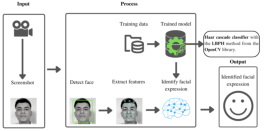
\includegraphics[frame,scale=0.5, width=\linewidth]{figs/Figure_3}
							\caption{Método para el reconocimiento de expresiones faciales utilizado en el sistema Torddis.\label{fig:FacialExpression}}
						\end{figure} 
						
					\paragraph{\textbf{Métodos para la Detección de Sueño}}
						Los métodos para la detección de sueño requieren una imagen que contenga un rostro como entrada. Estos métodos realizan el preprocesamiento de la imagen para extraer los puntos característicos de los ojos y luego analizan si la persona tiene los ojos cerrados. La Tabla \ref{tab:sleep-detection-methods} enumera los métodos para la detección de sueño.
						
						\begin{table}[hbt]
							\centering
							\caption{Métodos para la detección de sueño.}
							\label{tab:sleep-detection-methods}
							\begin{tabular}{p{0.35\textwidth}p{0.43\textwidth}p{0.10\textwidth}}
								\hline
								\multicolumn{1}{c}{\rule{0pt}{2.5ex}\textbf{Algoritmo}} & \multicolumn{1}{c}{\rule{0pt}{2.5ex}\textbf{\parbox{3cm}{Uso}}} & \multicolumn{1}{c}{\rule{0pt}{2.5ex}\textbf{Precisión}} \\ \hline
								MediaPipe Face Mesh & Detección de puntos característicos faciales con 468 puntos 3D \citep{Shanmugam2022Comparative}. & \multicolumn{1}{r}{99.87\%} \\ 
								SVM & Seguimiento de ojos \citep{Altameem2021Early}. & \multicolumn{1}{r}{83.25\%} \\
								CNN & Entrenado con 4 gestos, como ojos abiertos, ojos cerrados, bostezando y no bostezando \citep{Diagram2023Software}. & \multicolumn{1}{r}{80.00\%} \\ \hline
							\end{tabular}
						\end{table}
					
					\paragraph{\textbf{Métodos para el Reconocimiento de Objetos}}			
						La visión por computadora permite la detección automática de la estructura y propiedades de un posible mundo dinámico tridimensional. Primero, se requiere una imagen de entrada que contenga uno o más objetos. Luego, se realiza el preprocesamiento de la imagen para extraer características de la imagen segmentada. La Tabla \ref{tab:object-recognition} describe una lista de algoritmos para el reconocimiento de objetos.
						
						\begin{table}[ht!]
							\caption{Algoritmos para el reconocimiento de objetos.}
							\label{tab:object-recognition}
							\centering
							\begin{tabular}{p{0.1\textwidth}p{0.32\textwidth}p{0.39\textwidth}p{0.8\textwidth}}
								\hline
								\multicolumn{1}{l}{\textbf{Algoritmo}} & \multicolumn{1}{l}{\textbf{Tecnología e Implementación}} & \multicolumn{1}{l}{\textbf{Uso}} & \multicolumn{1}{l}{\textbf{Precisión}} \\ \hline
								YOLO & YOLOv4 & Reconocimiento de objetos \citep{Liu2021Objetcs}. & \multicolumn{1}{r}{73.01\%} \\
								Sequential TensorFlow & Keras & Clasificación y detección de imágenes aéreas \citep{Sudharshan2018Object}. & \multicolumn{1}{r}{96.00\%} \\ \hline
							\end{tabular}
						\end{table}
						En base a la información de la Tabla \ref{tab:object-recognition}, el algoritmo seleccionado fue \textit{Sequential} de la biblioteca \textit{TensorFlow} en combinación con \textit{Keras} debido a su precisión, rendimiento óptimo, facilidad de entrenamiento y uso generalizado para el reconocimiento de objetos en tiempo real. MobileNetV2 combinado con SSD se descartó debido a su menor precisión en el reconocimiento de objetos en comparación con otros. Además, YOLO fue descartado debido al alto consumo de GPU (Unidad de Procesamiento Gráfico) requerido para su correcto funcionamiento.
					
					\paragraph{\textbf{Procedimiento para el Reconocimiento de Objetos}}
						Este método consiste en los siguientes pasos:
						\begin{enumerate}
							\item Se toma una fotografía para capturar los objetos ubicados en el escritorio o el área donde el niño está trabajando.
							\item Se realiza el preprocesamiento de la imagen, seguido de la segmentación en partes correspondientes a los posibles objetos.
							\item Se lleva a cabo la extracción de características en la imagen segmentada.
							\item Finalmente, las características extraídas se comparan con un modelo computacional, que fue entrenado con un conjunto de imágenes que contienen los objetos que se espera reconocer.
						\end{enumerate}
						
						La visión por computadora permite la detección automática de la estructura y propiedades de un posible mundo dinámico en tres dimensiones, basándose en una o más imágenes bidimensionales del mundo \citep{Cruz2013}. La Figura \ref{fig:ObjectRecognition} ilustra el método de reconocimiento de objetos utilizado en la implementación del sistema Torddis.
						
						\begin{figure}[h]
							\centering
							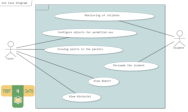
\includegraphics[frame,scale=0.5, width=\linewidth]{figs/Figure_4}
							\caption{Método para el reconocimiento de objetos utilizado en el sistema Torddis.\label{fig:ObjectRecognition}}
						\end{figure} 
			
			\subsubsection{Diseño de la Capa Tecnológica}
				Posterior a la obtención de los requisitos de Torddis, se procedió a diseñar su arquitectura (ver figura \ref{fig:TorddisArchitecture}). Además, con la ayuda de la herramienta TDDT4IoTS \citep{Guerrero2024Test} se diseño el dispositivo IoT (ver \ref{fig:TorddisDevice}). En resumen, tanto la arquitectura del dispositivo como la arquitectura del software se diseñaron utilizando la herramienta TDDT4IoTS.
				
				\begin{figure}[hbt!]
					\centering
					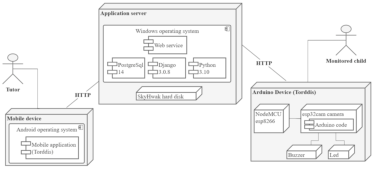
\includegraphics[frame,scale=0.5, width=\linewidth]{figs/Figure_5}
					\caption{Arquitectura del sistema Torddis. \label{fig:TorddisArchitecture}}
				\end{figure} 
				
				\begin{figure}[hbt!]
					\centering
					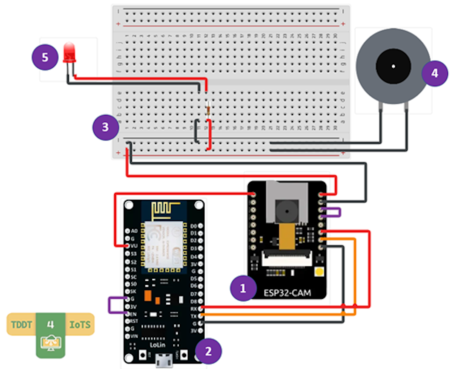
\includegraphics[frame,scale=0.5, width=\linewidth]{figs/Figure_6}
					\caption{Diseño del dispositivo del sistema Torddis. \label{fig:TorddisDevice}}
				\end{figure} 
				
				Para el diseño del dispositivo se utilizaron los componentes:
				\begin{enumerate}
					\item Placa ESP32 CAM
					\item Placa ESP8266 NODE MCU
					\item Placa Protoboard
					\item Buzzer pasivo
					\item Led de color rojo
				\end{enumerate}
			
			\subsubsection{Análisis Detallado de Requisitos}
				Con la arquitectura y las funcionalidades a grano grueso del sistema ya definidas, se procedió a obtener los requisitos a grano fino para una implementación exitosa de Torddis. En la figura \ref{fig:Fine-GrainedUseCas} se muestra el diagrama de casos de uso que muestran el dominio más claro del problema.
				
				\begin{figure}[hbt!]
					\centering
					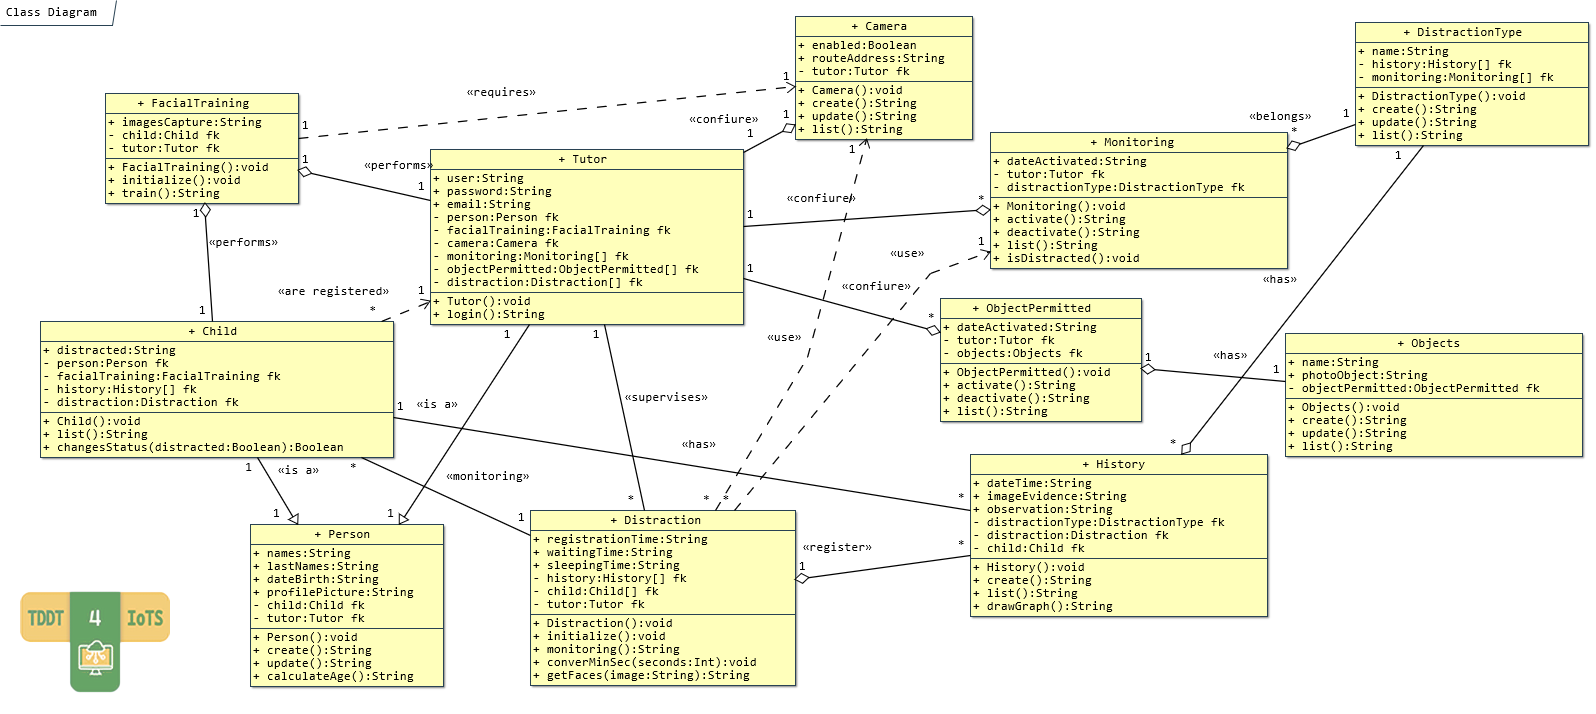
\includegraphics[frame,scale=0.5, width=\linewidth]{figs/Figure_7}
					\caption{Diagrama de casos de uso a grano fino del sistema Torddis. \label{fig:Fine-GrainedUseCas}}
				\end{figure} 
				
				Así mismo en la tabla \ref{tab:use-case-register-device} se muestran los casos de uso ampliados a gran detalle para que los desarrolladores implementen la lógica de negocios complementaria para que el sistema cumpla con las especificaciones.
				
				\begin{table}[hbt!]
					\centering
					\caption{Caso de Uso: Registrar Dispositivo Torddis}
					\label{tab:use-case-register-device}
					\begin{tabularx}{\textwidth}{|l|X|}
						\hline
						\textbf{Caso de Uso} & Registrar dispositivo Torddis \\ \hline
						\textbf{Descripción} & El tutor ingresa la dirección MAC del dispositivo Torddis. El sistema registra el dispositivo Torddis en la base de datos y muestra un mensaje indicando lo sucedido. \\ \hline
						\textbf{Actores} & Tutor \\ \hline
						\textbf{Condiciones Previas} & Usuario autenticado como tutor. \\ \hline
						\textbf{Condiciones Posteriores} & Dispositivo Torddis del tutor vinculado. \\ \hline
						\textbf{Flujo Normal} & 
						\begin{enumerate}
							\item El caso de uso comienza cuando el tutor accede a la interfaz para vincular dispositivo.
							\item El sistema muestra el formulario con los controles para vincular el dispositivo: dirección MAC del dispositivo.
							\item El tutor ingresa la dirección MAC del dispositivo y selecciona la opción de guardar (ver Alt 1).
							\item El sistema almacena los datos en la base de datos (ver E1).
							\item El sistema retroalimenta sobre el éxito de la operación.
							\item Este caso de uso termina cuando el sistema muestra la interfaz de entrenamiento facial.
						\end{enumerate} \\ \hline
						\textbf{Flujos Alternativos} & 
						\textbf{Alt 1.} El tutor no desea registrar el dispositivo Torddis:
						\begin{enumerate}
							\item[3.] Este caso de uso termina cuando el tutor cancela la operación.
						\end{enumerate} \\ \hline
						\textbf{Excepciones} & 
						\textbf{E1.} Error al registrar el dispositivo Torddis:
						\begin{enumerate}
							\item[4.] El sistema muestra un mensaje: \textit{Error al registrar el dispositivo Torddis, por favor intente nuevamente.}
							\item[5.] El tutor reanuda el paso 3 del flujo normal.
						\end{enumerate} \\ \hline
					\end{tabularx}
				\end{table} 
			
			\subsubsection{Generación y Refinamiento de Modelos}
				Entre las herramientas de modelado del sistema  se utilizaron los modelos de estructura como son los diagramas de clases. Este diagrama de clases )ver figura \ref{fig:ClassDiagram}) fue obtenido directamente de la herramienta usada \citep{Guerrero2024Test}.
				
				\begin{figure}[hbt!]
					\centering
					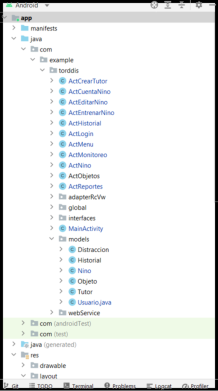
\includegraphics[frame,scale=0.5, width=\linewidth]{figs/Figure_8}
					\caption{Diagrama de clases del sistema Torddis.\label{fig:ClassDiagram}}
				\end{figure} 
				
				Además, se obtuvieron y refinaron los modelos computacionales de IA para monitorizar los eventos de los tutorados según los parámetros de distracción especificados, ajustando configuraciones como el número de capas ocultas y las épocas de entrenamiento del modelo.
			
			\subsubsection{Generación de Pruebas}
				Las pruebas unitarias fueron generadas utilizando la herramienta TDDT4IoTS. Las pruebas de integración fueron ejecutadas manualmente por los desarrolladores, cuyas especificaciones fueron obtenidas desde el diseño de la arquitectura del sistemas, y complementadas más delante en las etapas de \textit{generación y refinamiento de modelos}.
				
				Las Tablas \ref{tab:create-tutor-account-test-case}, \ref{tab:login-test-case}, \ref{tab:face-training-test-case}, \ref{tab:device-registration-test-case}, y \ref{tab:configure-object-usage-test-case} muestran algunos de los casos de prueba de sistema que en la secuencia lógica fueron ejecutados por el equipo de desarrollo. Similares casos de prueba en la secuencia lógica que el usuario requería ejecutar sirvieron como casos de prueba de aceptación. Con este último tipo de pruebas los interesados verificaron que Torddis cumple con los requisitos especificados \citep{Sciarra2024Smash}.
				
				\begin{table}[hbt!]
					\centering
					\caption{Caso de prueba para la creación de la cuenta de tutor.}
					\label{tab:create-tutor-account-test-case}
					\begin{tabularx}{\textwidth}{l X}
						\toprule
						\textbf{Código del Caso de Prueba:} & PU-1 \\
						\textbf{Nombre del Caso de Prueba:} & Creación de Cuenta de Tutor \\
						\textbf{Resultado Esperado:} & Crear con éxito una cuenta de tutor \\
						\midrule
						\multicolumn{2}{c}{\textbf{Procedimiento del Caso de Prueba}} \\
						\midrule
						\multicolumn{1}{c}{\textbf{No.}} & \textbf{Descripción del Paso} \\
						\midrule
						\multicolumn{1}{c}{1} & Abrir la aplicación móvil. \\
						\multicolumn{1}{c}{2} & Seleccionar la opción "Registrarse". \\
						\multicolumn{1}{c}{3} & Ingresar los datos de registro.
						\begin{itemize}
							\item Nombre: Carlos Iván
							\item Apellidos: Almeida Dueñas
							\item Correo electrónico: carlos.almeida2017@utec.edu.ec
							\item Fecha de nacimiento: 10/01/2000
							\item Nombre de usuario: calmeidad
							\item Contraseña: XXXXXX
						\end{itemize}\\
						\multicolumn{1}{c}{4} & Seleccionar la opción "Crear Cuenta". \\
						\bottomrule
					\end{tabularx}
				\end{table}
				
				\begin{table}[hbt!]
					\centering
					\caption{Caso de prueba para iniciar sesión.}
					\label{tab:login-test-case}
					\begin{tabularx}{\textwidth}{l X}
						\toprule
						\textbf{Código del Caso de Prueba:} & PU-2 \\
						\textbf{Nombre del Caso de Prueba:} & Inicio de Sesión \\
						\textbf{Resultado Esperado:} & Iniciar sesión exitosamente con una cuenta de tutor \\ \midrule
						\multicolumn{2}{c}{\textbf{Procedimiento del Caso de Prueba}} \\ \midrule
						\multicolumn{1}{c}{\textbf{No.}} & \textbf{Descripción del Paso} \\ \midrule
						\multicolumn{1}{c}{1} & Ingresar las credenciales de inicio de sesión.
						\begin{itemize}
							\item Nombre de usuario: calmeidad
							\item Contraseña: XXXXXX
						\end{itemize} \\
						\multicolumn{1}{c}{2} & Seleccionar la opción "Iniciar Sesión". \\
						\multicolumn{1}{c}{3} & La aplicación móvil muestra la pantalla del menú del usuario tutor. \\
						\bottomrule
					\end{tabularx}
				\end{table}
				
				\begin{table}[hbt!]
					\centering
					\caption{Caso de prueba para el entrenamiento facial.}
					\label{tab:face-training-test-case}
					\begin{tabularx}{\textwidth}{l X}
						\toprule
						\textbf{Código del Caso de Prueba:} & PU-3 \\
						\textbf{Nombre del Caso de Prueba:} & Entrenamiento Facial \\
						\textbf{Resultado Esperado:} & Realizar con éxito el entrenamiento facial para un estudiante\\
						\midrule
						\multicolumn{2}{c}{\textbf{Procedimiento del Caso de Prueba}} \\
						\midrule
						\multicolumn{1}{c}{\textbf{No.}} & \textbf{Descripción del Paso} \\
						\midrule
						\multicolumn{1}{c}{1} & Ingresar al módulo "Niño" de la aplicación. \\
						\multicolumn{1}{c}{2} & Seleccionar la opción "Entrenar" para un niño. \\
						\multicolumn{1}{c}{3} & Registrar un dispositivo (ver caso de prueba Tabla \ref{tab:device-registration-test-case}). \\
						\multicolumn{1}{c}{4} & Seleccionar la opción "Entrenar". \\
						\multicolumn{1}{c}{5} & Colocar el rostro del niño frente a la cámara del dispositivo y esperar a que se complete el proceso de entrenamiento facial. \\
						\bottomrule
					\end{tabularx}
				\end{table}
				
				\begin{table}[hbt!]
					\centering
					\caption{Caso de prueba para el registro del dispositivo.}
					\label{tab:device-registration-test-case}
					\begin{tabularx}{\textwidth}{l X}
						\toprule
						\textbf{Código del Caso de Prueba:} & PU-4 \\
						\textbf{Nombre del Caso de Prueba:} & Registro del Dispositivo \\
						\textbf{Resultado Esperado:} & Registrar con éxito el dispositivo en la aplicación móvil \\
						\midrule
						\multicolumn{2}{c}{\textbf{Procedimiento del Caso de Prueba}} \\
						\midrule
						\multicolumn{1}{c}{\textbf{No.}} & \textbf{Descripción del Paso} \\
						\midrule
						\multicolumn{1}{c}{1} & Seleccionar la opción "Registrar Dispositivo". \\
						\multicolumn{1}{c}{2} & Ingresar la dirección IP del dispositivo. \\
						\multicolumn{1}{c}{3} & Seleccionar la opción "Guardar". \\
						\bottomrule
					\end{tabularx}
				\end{table}
				
				\begin{table}[hbt!]
					\centering
					\caption{Caso de prueba para configurar el uso de objetos.}
					\label{tab:configure-object-usage-test-case}
					\begin{tabularx}{\textwidth}{l X}
						\toprule
						\textbf{Código del Caso de Prueba:} & PU-5 \\
						\textbf{Nombre del Caso de Prueba:} & Configuración del Uso de Objetos \\
						\textbf{Resultado Esperado:} & Configurar con éxito el uso de objetos \\
						\midrule
						\multicolumn{2}{c}{\textbf{Procedimiento del Caso de Prueba}} \\
						\midrule
						\multicolumn{1}{c}{\textbf{No.}} & \textbf{Descripción del Paso} \\
						\midrule
						\multicolumn{1}{c}{1} & Ingresar al módulo "Objetos" de la aplicación. \\
						\multicolumn{1}{c}{2} & Buscar el objeto que se desea activar/desactivar. \\
						\multicolumn{1}{c}{3} & Seleccionar el control de interruptor de un objeto para activarlo/desactivarlo. \\
						\bottomrule
					\end{tabularx}
				\end{table}

			\subsubsection{Generación y Refinamiento de Software}
				En esta etapa se escribió el código del software basándose en los modelos generados y las pruebas tanto unitarias como de integración. Se utilizó el lenguaje de programación Python con la herramienta Visual Studio Code \citep{Microsoft2024Visual} para desarrollar los webs services, Java como lenguaje de programación con IDE Android Studio \citep{Android2024Android} para la aplicación móvil y lenguaje C++ en IDE Arduino \citep{Arduino2024Software} para configurar los componentes de hardware IoT del dispositivo de TORDDIS.
				
				El software fue generado usando la herramienta TDDT4IoTS \citep{Guerrero2024Test}, y luego completado manualmente por los desarrolladores. El mismo equipo de desarrolladores fueron los encargados de entregar el software probado y funcionando. En resumen, en esta etapa se obtuvo una versión del software por cada entregable probado y funcionando.
			
			\subsubsection{Despliegue de Software y Hardware}
				Los componentes de la aplicación móvil y finalmente la aplicación móvil en su conjunto fue desplegada en un Smartphone con Android versión 13 marca Xiaomi modelo Note 10 Pro. Aunque, la aplicación móvil puede ser desplegada en cualquier Smartphone Android de la versión 13 en adelante.
				
				La Figura \ref{fig:Torddis} muestra capturas de pantalla tanto de la aplicación móvil como del dispositivo Torddis, destacando su diseño intuitivo y las funciones clave para la monitorización en tiempo real de las distracciones de los estudiantes. Además, se muestra el dispositivo IoT, integrando tecnologías de reconocimiento facial y detección de objetos, proporcionando un apoyo integral para mejorar la concentración académica en el hogar.
				
				La Figura \ref{fig:TorddisApp}a muestra las diferentes opciones disponibles para el tutor, mientras que la Figura \ref{fig:TorddisApp}b muestra la lista de estudiantes bajo la supervisión de un tutor. Por otro lado, la Figura \ref{fig:TorddisApp}c muestra el dispositivo del sistema Torddis.
				
				\begin{figure}[h]
					\centering
					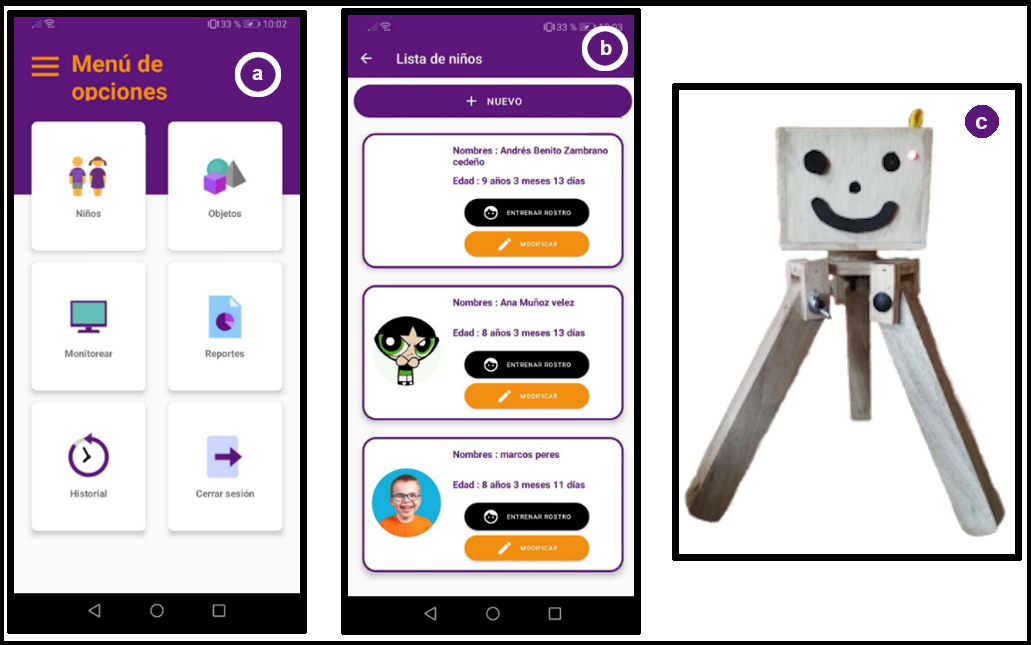
\includegraphics[width=\linewidth]{figs/Figure_9}
					\caption{Capturas de pantalla de la aplicación móvil y dispositivo del sistema Torddis.\label{fig:TorddisApp}} 
				\end{figure}
				
			\subsubsection{Evaluación de los Entregables}
				Cada entregable (aplicación móvil y dispositivo) fueron evaluados por el usuario en un ambiente ideal.
				La Figura \ref{fig:ConfigEvaluation} muestra la configuración del entorno utilizado para evaluar el sistema Torddis. El tutorado está sentado en un escritorio realizando actividades académicas mientras es monitorizado por el sistema Torddis.
				
				\begin{figure}[h]
					\centering
					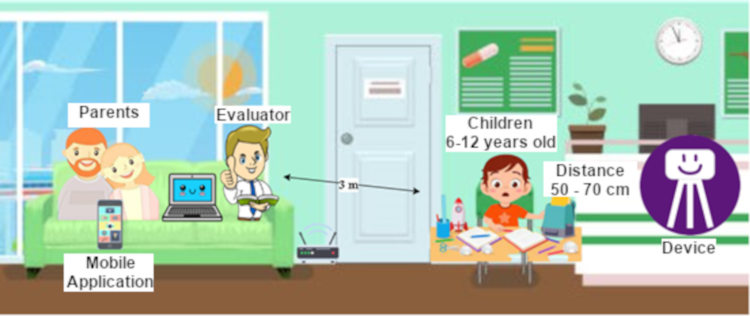
\includegraphics[width=\linewidth]{figs/Figure_10}
					\caption{Configuración del entorno para la evaluación del sistema Torddis. \label{fig:ConfigEvaluation}} 
				\end{figure}
				
				El sistema tiene la capacidad de monitorizar la concentración y las distracciones que puede tener el tutorado. El dispositivo se coloca a una distancia de entre 50 y 70 cm del tutorado, para el correcto funcionamiento de la cámara que proporciona a las tecnologías de reconocimiento facial y de objetos las entradas necesarias. Cabe mencionar que, para el tutorado, este dispositivo está destinado a ser percibido como un adorno decorativo o juguete en su escritorio.
				
				Un evaluador (uno de los autores), se encuentra posicionado a unos 3 metros del niño, supervisando el funcionamiento del sistema a través de una laptop. Uno o ambos padres están presentes, utilizando la aplicación móvil integrada con el dispositivo para monitorizar la concentración del niño en tiempo real, así como consultar la información resultante del procesamiento de los datos recopilados y analizados.
				
				Esta configuración permitió una evaluación integral del sistema Torddis, asegurando que todos los involucrados (niños, padres y evaluadores) pudieran interactuar con la tecnología y proporcionar información valiosa sobre su efectividad en la monitorización y mejora de la concentración académica en un entorno controlado.
				
				Para la evaluación de las funcionalidades del sistema en conjunto se realizaron las pruebas de aceptación que se detallan en las tablas \ref{tab:create-tutor-account-test-case}, \ref{tab:login-test-case}, \ref{tab:face-training-test-case}, \ref{tab:device-registration-test-case}, y \ref{tab:configure-object-usage-test-case}.
				
				\subsubsection*{Evaluación de Usabilidad del Sistema Prototipo Desarrollado}
					La evaluación de la usabilidad del sistema Torddis se llevó a cabo para recopilar información sobre la experiencia general del usuario, centrándose específicamente en la facilidad de uso, la interfaz del sistema y la efectividad de las funciones proporcionadas. Esta evaluación integral tuvo como objetivo identificar fortalezas y áreas de mejora, asegurando que el sistema cumpla eficazmente con las necesidades de los usuarios. Las siguientes subsecciones detallan los datos demográficos de los participantes, sus experiencias, las tareas específicas realizadas durante la evaluación y los resultados del cuestionario SUS y de las preguntas abiertas (ver Apéndice \ref{Appendix:SUSQuestionarie}).
					
					\paragraph{\textbf{Datos Demográficos:}}
						Al inicio de la evaluación de usabilidad, se proporcionó un cuestionario demográfico para recopilar información sobre los tutores que participaron en la evaluación de usabilidad del sistema Torddis (ver Apéndice \ref{Appendix:DemographicSurvey}). El cuestionario demográfico arrojó los siguientes resultados:
						
						\begin{itemize}
							\item Se evaluaron un total de 12 familias: 8 madres y 4 padres, todos pertenecientes a la zona geográfica de Quevedo, Ecuador.
							\item La edad promedio de los participantes es de 39 años, con un rango de edad entre 25 y 65 años.
							\item El 58\% de los tutores solo completaron la educación primaria, mientras que el 42\% estudiaron hasta la educación secundaria.
						\end{itemize}
						
					\paragraph{\textbf{Acerca de la Monitorización:}}
						Una de las preguntas preliminares en la evaluación de usabilidad fue sobre la facilidad con la que pueden monitorizar a sus hijos de primaria mientras realizan sus tareas escolares (ver Figura \ref{fig:previous-questions}). La mayoría de los tutores respondieron que el proceso de monitorización de la distracción de los niños es una tarea compleja. La Figura \ref{fig:monitoring-process} muestra los resultados detallados. Otra pregunta preliminar fue sobre la frecuencia con la que necesitaban monitorizar a sus hijos mientras realizaban actividades escolares. La mayoría de los tutores indicaron que debían hacerlo constantemente. Para respuestas más detalladas, véase la Figura \ref{fig:monitoring-frequency}. Finalmente, los tutores indicaron que, entre las estrategias que utilizan para mantener a sus estudiantes concentrados en sus actividades escolares, están las llamadas de atención (regaños), los consejos motivacionales y las recompensas, tales como dulces, juguetes, paseos al parque, comidas favoritas, y así sucesivamente (ver Figura \ref{fig:concentration-strategies}).
						
						\begin{figure}[hbt!]
							\centering
							\begin{minipage}{0.45\textwidth}
								\centering
								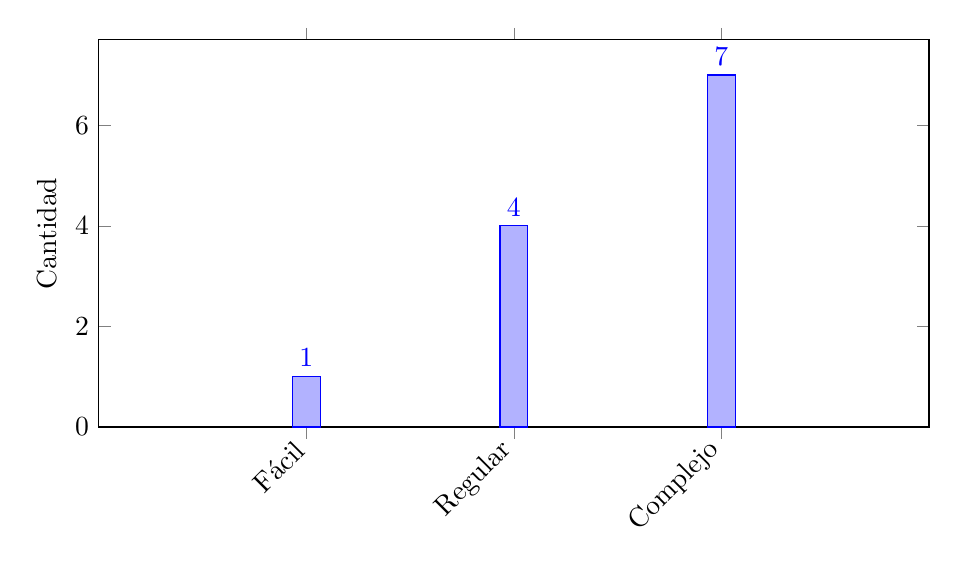
\begin{tikzpicture}
									\begin{axis}[
										ybar,
										width=\textwidth,
										height=6.5cm,
										symbolic x coords={Fácil, Regular, Complejo},
										xtick=data,
										ylabel={Cantidad},
										ymin=0,
										nodes near coords,
										enlarge x limits=0.5,
										x tick label style={rotate=45, anchor=east}
										]
										\addplot coordinates {(Fácil, 1) (Regular, 4) (Complejo, 7)};
									\end{axis}
								\end{tikzpicture}
								\subcaption{Facilidad del proceso de monitorización.}
								\label{fig:monitoring-process}
							\end{minipage}
							\vspace{5mm}
							\begin{minipage}{0.45\textwidth}
								\centering
								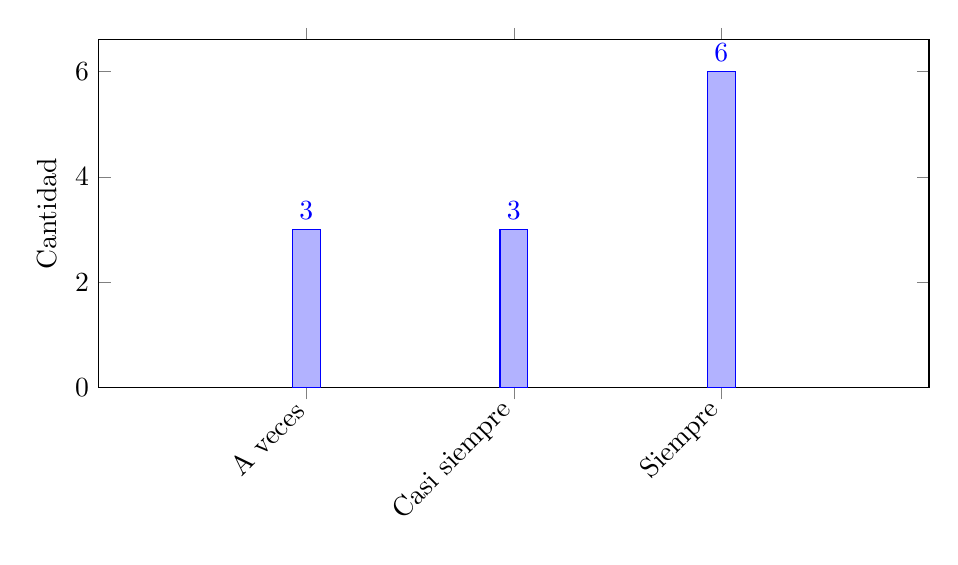
\begin{tikzpicture}
									\begin{axis}[
										ybar,
										width=\textwidth,
										height=6cm,
										symbolic x coords={A veces, Casi siempre, Siempre},
										xtick=data,
										ylabel={Cantidad},
										ymin=0,
										nodes near coords,
										enlarge x limits=0.5,
										x tick label style={rotate=45, anchor=east}
										]
										\addplot coordinates {(A veces, 3) (Casi siempre, 3) (Siempre, 6)};
									\end{axis}
								\end{tikzpicture}
								\subcaption{Frecuencia de monitorización.}
								\label{fig:monitoring-frequency}
							\end{minipage}
							\begin{minipage}{0.45\textwidth}
								\centering
								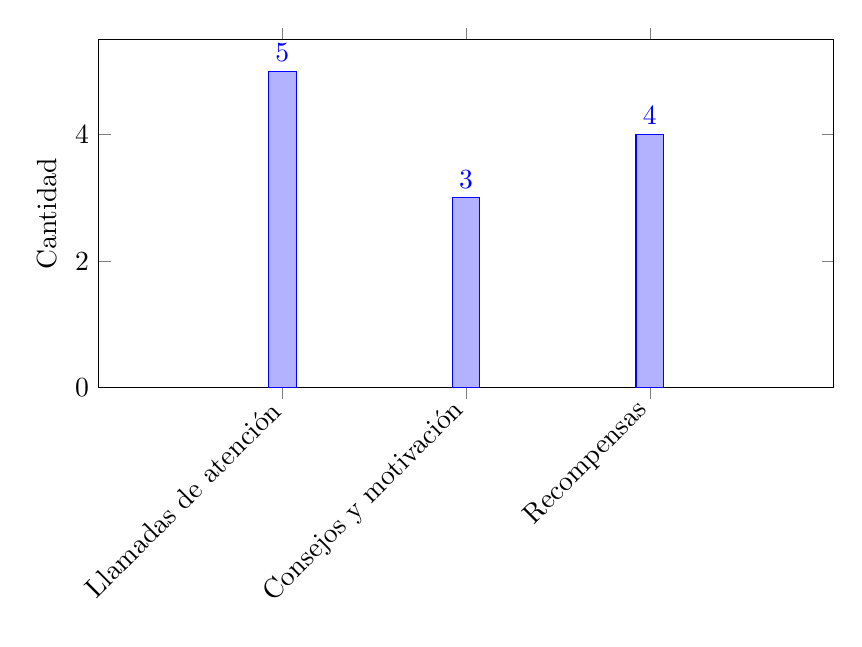
\begin{tikzpicture}
									\begin{axis}[
										ybar,
										height=6cm,
										width=0.9\textwidth,
										symbolic x coords={Llamadas de atención, Consejos y motivación, Recompensas},
										xtick=data,
										ylabel={Cantidad},
										ymin=0,
										nodes near coords,
										enlarge x limits=0.5,
										x tick label style={rotate=45, anchor=east}
										]
										\addplot coordinates {(Llamadas de atención, 5) (Consejos y motivación, 3) (Recompensas, 4)};
									\end{axis}
								\end{tikzpicture}
								\subcaption{Estrategias para lograr la concentración.}
								\label{fig:concentration-strategies}
							\end{minipage}
							\caption{Resultados de preguntas realizadas a los padres sobre el proceso de monitorización de sus hijos de primaria mientras hacen sus tareas.}
							\label{fig:previous-questions}
						\end{figure}
					
					\paragraph{\textbf{Tareas para los Usuarios Participantes:}}
						Las tareas que los tutores realizaron durante la evaluación fueron las siguientes:
						
						\begin{enumerate}
							\item Conectar el dispositivo Torddis a la fuente de alimentación y colocarlo en el escritorio donde el niño se sentará para realizar una tarea.
							\item Crear una cuenta de usuario tutor en la aplicación móvil.
							\item Iniciar sesión en la aplicación móvil.
							\item Registrar al niño que será monitoreado.
							\item Registrar el dispositivo Torddis en la aplicación móvil utilizando la dirección IP proporcionada en una etiqueta adherida al dispositivo.
							\item Realizar el entrenamiento facial para el niño registrado.
							\item Activar y/o desactivar los objetos que se monitorizarán en la sección correspondiente de la aplicación móvil.
							\item Asignar una tarea al niño mientras es monitoreado por el dispositivo Torddis: colorear un mandala.
							\item Activar el reconocimiento de cada parámetro de distracción en la sección de monitorización de la aplicación móvil.
							\item Dejar al niño solo, sin la presencia de un adulto, durante 6 minutos.
							\item Activar y/o desactivar la transmisión de video desde el dispositivo Torddis.
							\item Navegar por el historial de los parámetros de distracción monitoreados en el niño.
							\item Visualizar un informe con gráficos que representan los parámetros de distracción detectados para el niño monitoreado.
						\end{enumerate}
					
					\paragraph{\textbf{Resultados del Cuestionario System Usability Scale:}}
						Los resultados analizados en esta sección corresponden a las respuestas del cuestionario SUS (ver Apéndice \ref{Appendix:LikertScale}) proporcionado a los 12 tutores. Después de tabular los datos obtenidos, la Figura \ref{fig:sus-questionnaire} muestra que la media de los datos recopilados es 81.46\% con una desviación estándar de 11.65. Según los adjetivos (Peor imaginable, Pobre, OK, Bueno, Excelente, Mejor imaginable) propuestos por \cite{Bangor2008AnEmpirical} para evaluar cualitativamente la usabilidad de un sistema basado en la media alcanzada, es evidente que Torddis tiene un nivel de usabilidad "Bueno" según los tutores evaluados.
						
						\begin{figure}[hbt!]
							\centering
							\begin{tikzpicture}
								\begin{axis}[
									scatter/classes={
										a={mark=*,blue}
									},
									width=12cm,
									height=8cm,
									xlabel={Participante},
									ylabel={Evaluación},
									ymin=40, ymax=100,
									xmin=0, xmax=13,
									xtick={1,2,3,4,5,6,7,8,9,10,11,12},
									xticklabels={1,2,3,4,5,6,7,8,9,10,11,12},
									ytick={40,60,80,100},
									nodes near coords,
									every node near coord/.append style={font=\footnotesize, /pgf/number format/fixed},
									legend style={at={(0.5,-0.15)}, anchor=north, legend columns=-1},
									enlarge x limits=0.05,
									]
									\addplot[
									scatter,
									only marks,
									scatter src=explicit symbolic,
									visualization depends on=\thisrow{Evaluation} \as \label
									] table[meta=class,x=Participant,y=Evaluation] {
										Participant Evaluation class
										1 90.00 90.00
										2 95.00 95.00
										3 72.50 72.50
										4 60.00 60.00
										5 85.00 85.00
										6 67.50 67.50
										7 92.50 92.50
										8 67.50 67.50
										9 82.50 82.50
										10 85.00 85.00
										11 92.50 92.50
										12 87.50 87.50
									};
									
									% Línea de promedio
									\addplot [
									color=orange,
									thick,
									mark=none
									] coordinates {(0,\average) (13,\average)};
									
									% Línea de desviación estándar superior
									\addplot [
									color=orange,
									thick,
									dashed,
									mark=none
									] coordinates {(0,\upperlimit) (13,\upperlimit)};
									
									% Línea de desviación estándar inferior
									\addplot [
									color=orange,
									thick,
									dashed,
									mark=none
									] coordinates {(0,\lowerlimit) (13,\lowerlimit)};
									
									\legend{Participante, Promedio SUS, Desv. Estándar}
								\end{axis}
							\end{tikzpicture}
							\caption{Datos del cuestionario SUS por tutor con evaluación promedio y desviación estándar.}
							\label{fig:sus-questionnaire}
						\end{figure}
						
					\paragraph{\textbf{Resultados del Cuestionario de Preguntas Abiertas:}}
						Al final del cuestionario SUS, los tutores respondieron 8 preguntas abiertas (ver Apéndice \ref{Appendix:OpenQuestions}) para proporcionar sus opiniones personales.
						
						La primera pregunta fue "¿Cuál es su opinión general sobre el sistema?", a la que algunos tutores respondieron que apoya la concentración de los estudiantes, y otros dijeron que tiene un diseño agradable. Los resultados se muestran en la Figura \ref{fig:AboutTorddis}. La segunda pregunta abierta que respondieron los tutores fue "¿Le gustaron los sonidos y/o luces que utiliza Torddis?". La mayoría de los tutores presentaron una opinión favorable a esta pregunta, ya que creen que las alertas luminosas ayudan a mantener al estudiante despierto y están satisfechos con las alarmas sonoras (ver Figura \ref{fig:SoundAndLigth}).
						
						\begin{figure}[hbt!]
							\centering
							\begin{minipage}{0.45\textwidth}
								\centering
								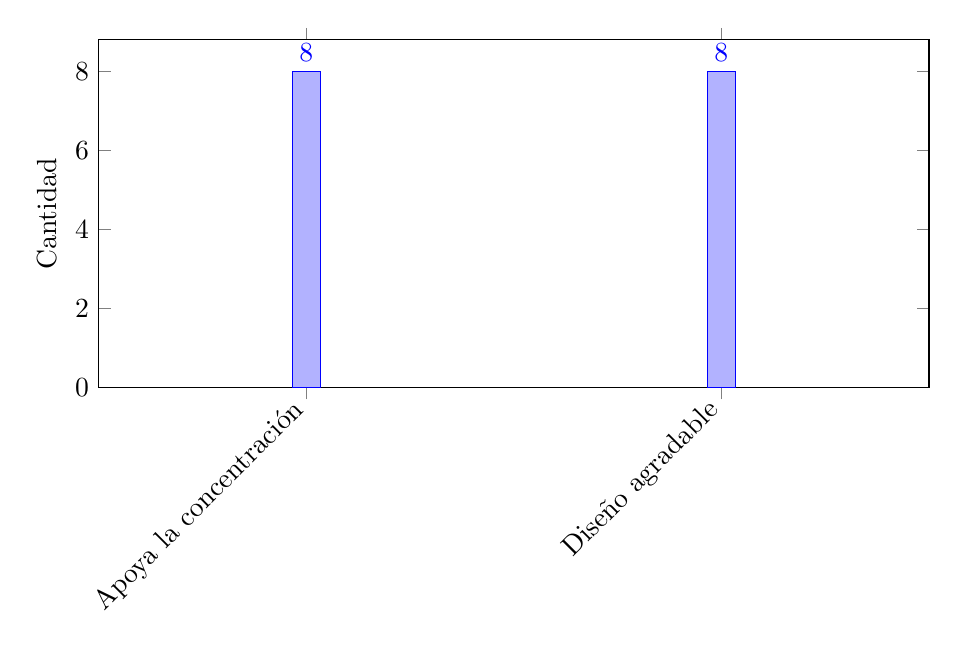
\begin{tikzpicture}
									\begin{axis}[
										ybar,
										width=\textwidth,
										height=6cm,
										symbolic x coords={Apoya la concentración, Diseño agradable},
										xtick=data,
										ylabel={Cantidad},
										ymin=0,
										nodes near coords,
										enlarge x limits=0.5,
										x tick label style={rotate=45, anchor=east}
										]
										\addplot coordinates {(Apoya la concentración, 8) (Diseño agradable, 8)};
									\end{axis}
								\end{tikzpicture}
								\subcaption{Opinión general sobre el sistema Torddis.}
								\label{fig:AboutTorddis}
							\end{minipage}
							\vspace{5mm}
							\begin{minipage}{0.45\textwidth}
								\centering
								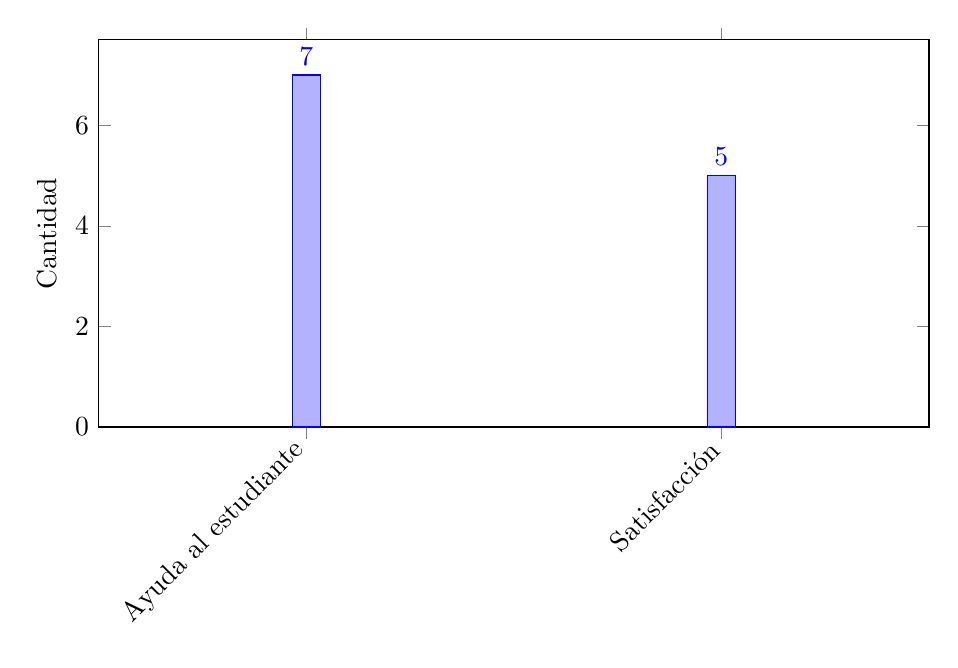
\begin{tikzpicture}
									\begin{axis}[
										ybar,
										width=\textwidth,
										height=6.5cm,
										symbolic x coords={Ayuda al estudiante, Satisfacción},
										xtick=data,
										ylabel={Cantidad},
										ymin=0,
										nodes near coords,
										enlarge x limits=0.5,
										x tick label style={rotate=45, anchor=east}
										]
										\addplot coordinates {(Ayuda al estudiante, 7) (Satisfacción, 5)};
									\end{axis}
								\end{tikzpicture}
								\subcaption{Alertas sonoras y luminosas del sistema.}
								\label{fig:SoundAndLigth}
							\end{minipage}
							\begin{minipage}{0.45\textwidth}
								\centering
								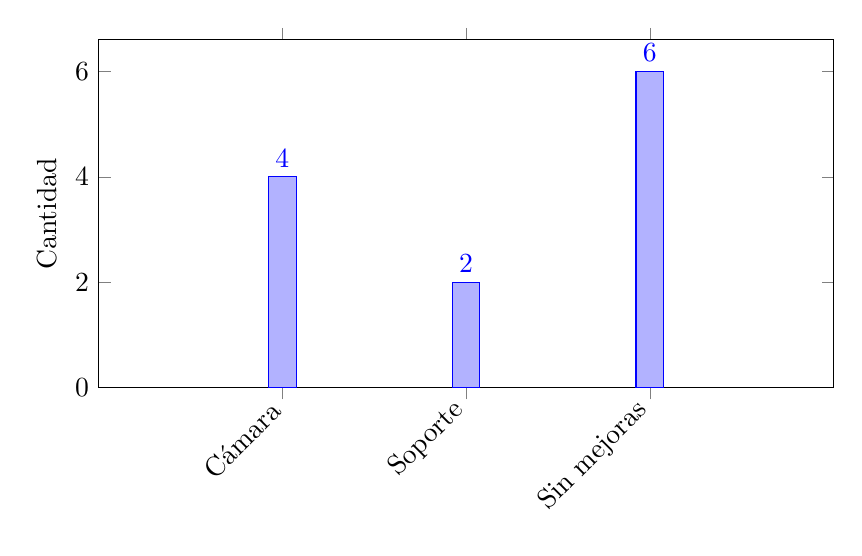
\begin{tikzpicture}
									\begin{axis}[
										ybar,
										height=6cm,
										width=0.9\textwidth,
										symbolic x coords={Cámara, Soporte, Sin mejoras},
										xtick=data,
										ylabel={Cantidad},
										ymin=0,
										nodes near coords,
										enlarge x limits=0.5,
										x tick label style={rotate=45, anchor=east}
										]
										\addplot coordinates {(Cámara, 4) (Soporte, 2) (Sin mejoras, 6)};
									\end{axis}
								\end{tikzpicture}
								\subcaption{Sugerencias para mejorar el sistema.}
								\label{fig:Improvements}
							\end{minipage}
							\begin{minipage}{0.45\textwidth}
								\centering
								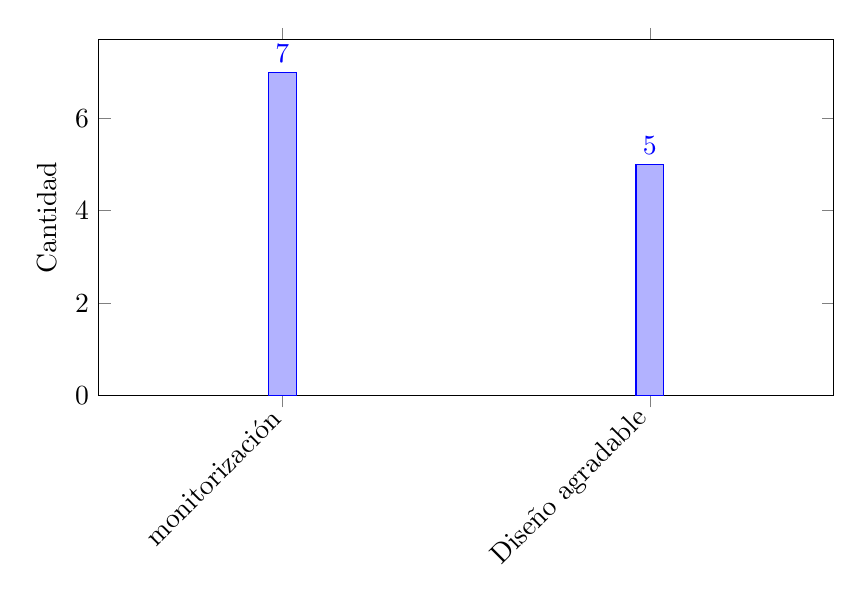
\begin{tikzpicture}
									\begin{axis}[
										ybar,
										height=6.1cm,
										width=0.9\textwidth,
										symbolic x coords={monitorización, Diseño agradable},
										xtick=data,
										ylabel={Cantidad},
										ymin=0,
										nodes near coords,
										enlarge x limits=0.5,
										x tick label style={rotate=45, anchor=east}
										]
										\addplot coordinates {(monitorización, 7) (Diseño agradable, 5)};
									\end{axis}
								\end{tikzpicture}
								\subcaption{Razones para recomendar el sistema.}
								\label{fig:ReasonsRecomend}
							\end{minipage}
							\caption{Resultados de preguntas realizadas a los padres sobre el proceso de monitorización de sus hijos de primaria usando Torddis mientras hacen sus tareas.}
							\label{fig:AnswerOfOpenQuestion}
						\end{figure}
						
						En las preguntas 3 ("¿Le gusta el diseño de la aplicación móvil Torddis? ¿Por qué?"), 4 ("¿Es adecuada la forma en que se visualizan los datos de monitorización de distracción de su hijo en la aplicación móvil Torddis? ¿Por qué?"), 5 ("¿Cree que este sistema ayudaría a mejorar la concentración de su hijo y mantenerlo informado mientras realiza sus tareas escolares? ¿Por qué?"), y 7 ("¿Estaría dispuesto a seguir usando el sistema Torddis?"), todos los tutores expresaron comentarios positivos. Manifestaron que les agrada el diseño de las vistas de la aplicación móvil, destacaron la organización de los datos históricos y los gráficos de informes, confirmaron que el sistema prototipo apoya eficazmente la concentración de los niños manteniéndolos informados cuando el niño se distrae, e indicaron su disposición a continuar usando el sistema Torddis.
						
						La pregunta 6 tenía como objetivo recopilar información sobre las mejoras que se podrían hacer a Torddis. Los comentarios obtenidos incluyen el uso de una cámara de mayor calidad y la mejora del soporte en el que se monta la cámara. Sin embargo, un alto porcentaje de usuarios mencionó que el dispositivo no necesita más mejoras. Estos resultados se muestran en la Figura \ref{fig:Improvements}. Por su parte, la pregunta 8 recopiló las razones por las que los evaluadores de Torddis recomendarían el uso de este sistema para la monitorización de estudiantes durante sus actividades escolares. La Figura \ref{fig:ReasonsRecomend} muestra las razones mencionadas por los tutores, incluyendo que les ayuda en la monitorización de sus estudiantes y su diseño agradable.
			\subsubsection*{Análisis de Reconocimiento}
				Esta subsección presenta los resultados de 14 pruebas realizadas utilizando el sistema Torddis, en las cuales se evaluaron cuatro tareas diferentes de reconocimiento: personas, expresiones faciales, presencia de sueño y objetos distractores. Cada prueba midió el tiempo en segundos que tomó reconocer el elemento correspondiente y registró si el reconocimiento fue exitoso o no. La Tabla \ref{tab:combined-recognition} muestra los datos recopilados para este análisis.
				
				\begin{table}[hbt!]
				\centering
				\caption{Resultados agregados de reconocimiento.}
				\label{tab:combined-recognition}
				\begin{tabularx}{\textwidth}{c >{\centering\arraybackslash}X c >{\centering\arraybackslash}X c >{\centering\arraybackslash}X c >{\centering\arraybackslash}X c}
					\toprule
					\textbf{No.} & \multicolumn{2}{c}{\textbf{Personas}} & \multicolumn{2}{c}{\textbf{Expresiones Faciales}} & \multicolumn{2}{c}{\textbf{Presencia de Sueño}} & \multicolumn{2}{c}{\textbf{Objetos Distractores}}\\
					\cline{2-9}
					& \textbf{Latencia} & \textbf{Logrado?} & \textbf{Latencia} & \textbf{Logrado?} & \textbf{Latencia} & \textbf{Logrado?} & \textbf{Latencia} & \textbf{Logrado?} \\
					\midrule
					1 & 0.57 & Sí & 1.50 & Sí & 5.10 & Sí & 0.00 & \textbf{No} \\
					2 & 0.60 & Sí & 1.20 & Sí & 3.50 & Sí & 1.68 & Sí \\
					3 & 0.00 & \textbf{No} & 0.70 & Sí & 0.00 & \textbf{No} & 0.00 & No \\
					4 & 0.78 & Sí & 1.30 & Sí & 3.68 & Sí & 1.79 & Sí \\
					5 & 1.02 & Sí & 0.78 & Sí & 2.24 & Sí & 0.00 & \textbf{No} \\
					6 & 0.88 & Sí & 1.01 & \textbf{No} & 2.63 & Sí & 1.98 & Sí \\
					7 & 0.53 & Sí & 1.23 & Sí & 0.00 & \textbf{No} & 1.73 & Sí \\
					8 & 1.20 & Sí & 0.97 & Sí & 2.03 & Sí & 2.05 & Sí \\
					9 & 0.76 & Sí & 1.05 & Sí & 4.09 & Sí & 1.77 & Sí \\
					10 & 1.20 & Sí & 0.70 & Sí & 3.36 & Sí & 1.91 & Sí \\
					11 & 0.69 & Sí & 1.99 & Sí & 4.69 & Sí & 4.27 & Sí \\
					12 & 0.82 & Sí & 1.83 & Sí & 3.29 & Sí & 2.69 & Sí \\
					13 & 0.93 & Sí & 1.68 & Sí & 3.14 & Sí & 2.81 & Sí \\
					14 & 0.58 & Sí & 1.76 & Sí & 3.45 & Sí & 2.94 & Sí \\
					\bottomrule
				\end{tabularx}
				\end{table}
				
				Los resultados de las pruebas de normalidad, se muestran en la Tabla \ref{table:PersonsNormality}.
				
				\begin{table}[h]
					\centering
					\caption{Análisis de normalidad de los tiempos de respuesta en el reconocimiento de personas.}
					\label{table:PersonsNormality}
					\begin{tabularx}{0.6\textwidth}{Xccc}
						\toprule
						\textbf{Detalle} & \textbf{Shapiro-Wilk} & \textbf{D'Agostino} & \textbf{Anderson-Darling}\\
						\midrule
						Estadístico & 0.9314 & 0.9445 &  0.3418 \\
						p-valor & 0.3188 & 0.1391 & 1\% al 15\% \\
						Conclusión & \(\checkmark\) & \(\checkmark\) & \(\checkmark\)\\
					\end{tabularx}
					\vspace{0.3em} % Espaciado entre la tabla y el pie
					\parbox{0.75\textwidth}{\footnotesize
						\(\checkmark\): Los datos siguen una distribución normal. p-valor para Anderson-Darling son los niveles de significancia.
					}
				\end{table}
				
				\begin{table}[h]
					\centering
					\caption{Análisis de normalidad de los tiempos de respuesta en el reconocimiento de expresiones faciales.}
					\label{FaceExpressionsNormality}
					\begin{tabularx}{0.6\textwidth}{Xccc}
						\toprule
						\textbf{Detalle} & \textbf{Shapiro-Wilk} & \textbf{D'Agostino} & \textbf{Anderson-Darling}\\
						\midrule
						Estadístico & 0.9402 & 1.7300 &  0.2937 \\
						p-valor & 0.4212 & 0.4211 & 1\% al 15\% \\
						Conclusión & \(\checkmark\) & \(\checkmark\) & \(\checkmark\)\\
					\end{tabularx}
					\vspace{0.3em} % Espaciado entre la tabla y el pie
					\parbox{0.75\textwidth}{\footnotesize
						\(\checkmark\): Los datos siguen una distribución normal. p-valor para Anderson-Darling son los niveles de significancia.
					}
				\end{table}
				
				\begin{table}[h]
					\centering
					\caption{Análisis de normalidad de los tiempos de respuesta en la detección de soñolencia.}
					\label{SleepingNormality}
					\begin{tabularx}{0.6\textwidth}{Xccc}
						\toprule
						\textbf{Detalle} & \textbf{Shapiro-Wilk} & \textbf{D'Agostino} & \textbf{Anderson-Darling}\\
						\midrule
						Estadístico & 0.9018 & 2.9592 &  0.5861 \\
						p-valor & 0.1198 & 0.2277 & 1\% al 5\% \\
						Conclusión & \(\checkmark\) & \(\checkmark\) & \(\checkmark\)\\
					\end{tabularx}
					\vspace{0.3em} % Espaciado entre la tabla y el pie
					\parbox{0.75\textwidth}{\footnotesize
						\(\checkmark\): Los datos siguen una distribución normal. p-valor para Anderson-Darling son los niveles de significancia.
					}
				\end{table}
				
				\begin{table}[h]
					\centering
					\caption{Análisis de normalidad de los tiempos de respuesta en la detección de Objetos distractores.}
					\label{ObjectNormality}
					\begin{tabularx}{0.6\textwidth}{Xccc}
						\toprule
						\textbf{Detalle} & \textbf{Shapiro-Wilk} & \textbf{D'Agostino} & \textbf{Anderson-Darling}\\
						\midrule
						Estadístico & 0.9033 & 0.2192 & 0.6563 \\
						p-valor & 0.1259 & 0.8962 & 1\% al 2.5\% \\
						Conclusión & \(\checkmark\) & \(\checkmark\) & \(\checkmark\)\\
					\end{tabularx}
					\vspace{0.3em} % Espaciado entre la tabla y el pie
					\parbox{0.75\textwidth}{\footnotesize
						\(\checkmark\): Los datos siguen una distribución normal. p-valor para Anderson-Darling son los niveles de significancia. \textbf{\textit{p-valor}} para Anderson-Darling es el nivel de significancia
					}
				\end{table}
				
				El nivel de significancia para las pruebas de Anderson-Darling es para el cual la hipótesis nula no se rechaza, es decir, se mantiene la hipótesis de que los datos siguen una distribución normal.
				
				\paragraph{Tiempo total de reconocimiento: }
					\begin{itemize}
					\item \textbf{Tiempo total de reconocimiento en segundos para todas las pruebas}: 
						\begin{itemize}
							\item Personas: 10.56 segundos
							\item Expresiones Faciales: 17.70 segundos
							\item Sueño: 41.20 segundos
							\item Objetos Distractores: 25.62 segundos
						\end{itemize}
					\item \textbf{Número de reconocimientos exitosos}:
						\begin{itemize}
							\item Personas: 13
							\item Expresiones Faciales: 13
							\item Sueño: 12
							\item Objetos Distractores: 11
						\end{itemize}
					\item \textbf{Número de fallos en el reconocimiento}:
						\begin{itemize}
							\item Personas: 1
							\item Expresiones Faciales: 1
							\item Sueño: 2
							\item Objetos Distractores: 3
						\end{itemize}
					\end{itemize}
				
				\paragraph{Tiempo Promedio de Reconocimiento: }
					El tiempo promedio para los reconocimientos exitosos se calculó para cada tarea de reconocimiento:
					
					\begin{itemize}
						\item \textbf{Personas}: \(\frac{10.56 \text{ segundos}}{13} \approx 0.81 \text{ segundos}\)
						\item \textbf{Expresiones Faciales}: \(\frac{17.70 \text{ segundos}}{13} \approx 1.36 \text{ segundos}\)
						\item \textbf{Sueño}: \(\frac{41.20 \text{ segundos}}{12} \approx 3.43 \text{ segundos}\)
						\item \textbf{Objetos Distractores}: \(\frac{25.62 \text{ segundos}}{11} \approx 2.33 \text{ segundos}\)
					\end{itemize}
					
				\paragraph{Tasa de Reconocimiento: }
					La tasa de reconocimiento se determinó para cada tarea como el porcentaje de reconocimientos exitosos sobre el total de pruebas:
				
					\begin{itemize}
						\item \textbf{Personas}: \(92.86\%\)
						\item \textbf{Expresiones Faciales}: \(92.86\%\)
						\item \textbf{Sueño}: \(85.71\%\)
						\item \textbf{Objetos Distractores}: \(78.57\%\)
					\end{itemize}
				
				\paragraph{Tiempos Mínimos y Máximos de Reconocimiento: }
					Tiempos mínimos y máximos de reconocimiento observados en las pruebas para cada tarea:
				
					\begin{itemize}
						\item \textbf{Personas}:
							\begin{itemize}
								\item Tiempo mínimo: 0.00 segundos (Prueba 3)
								\item Tiempo máximo: 1.20 segundos (Pruebas 8 y 10)
							\end{itemize}
						\item \textbf{Expresiones Faciales}:
							\begin{itemize}
								\item Tiempo mínimo: 0.70 segundos (Pruebas 3 y 10)
								\item Tiempo máximo: 1.99 segundos (Prueba 11)
							\end{itemize}
						\item \textbf{Sueño}:
							\begin{itemize}
								\item Tiempo mínimo: 0.00 segundos (Pruebas 3 y 7)
								\item Tiempo máximo: 5.10 segundos (Prueba 1)
							\end{itemize}
						\item \textbf{Objetos Distractores}:
							\begin{itemize}
								\item Tiempo mínimo: 0.00 segundos (Pruebas 1, 3 y 5)
								\item Tiempo máximo: 4.27 segundos (Prueba 11)
							\end{itemize}
					\end{itemize}
					
				\paragraph{Distribución de los Tiempos de Reconocimiento:}
					Los tiempos de reconocimiento para cada tarea varían, lo que indica una variabilidad en la respuesta del sistema. La mayoría de los tiempos de reconocimiento están dentro de un rango razonable, lo que sugiere una respuesta rápida y efectiva del sistema en la mayoría de los casos.
				
			\subsubsection{Mantenimiento}
				Esta fase no fue ejecutada debido al corto tiempo de desarrollo para cada entregable, y además para la evaluación del proyecto. Sin embargo, el sistema debe ser mantenido bajo las indicaciones de prevención y de vida útil de cada uno de los componentes para funcionar correctamente. La Tabla \ref{tab:maintenance-tasks} describe algunas tareas de mantenimiento tentativas. En general, el mantenimiento del sistema se debe considerar hacerlo de manera trimestral y semestral, aunque su frecuencia puede variar dependiendo del entorno en el que se lo use.
				
				\begin{table}[h]
					\centering
					\caption{Definición de tareas de mantenimiento.}
					\label{tab:maintenance-tasks}
					\begin{tabularx}{\textwidth}{cXcc}
						\toprule
						\textbf{No.} & \textbf{Tareas de Mantenimiento} & \textbf{Trimestral} & \textbf{Semestral} \\
						\midrule
						1 & Limpieza interna del dispositivo. & * & \\
						2 & Verificar si los componentes del dispositivo tienen alguna imperfección o daño. & & * \\
						3 & Comprobar conexiones de cables, estado de los cables, conectores, etc. & & * \\
						4 & Probar el funcionamiento del zumbador y los LED. & * & \\
						5 & Probar el sistema informático (servidor de aplicaciones web, servicios web, aplicación móvil, dispositivo IoT). & & * \\
						\bottomrule
					\end{tabularx}
				\end{table}
				Los tiempos para el mantenimiento preventivo se consideran de acuerdo al componente con tiempo de vida útil. Así mismo¡, el mantenimiento correctivo por cada componente físico del sistema se debe realizar antes que la vida útil del componente llegue a su límite. La vida útil de cada uno de los componentes se muestra en la Tabla \ref{tab:ShelfLife}. El tiempo de vida útil de las resistencias se espera que sea significativamente mayor al del componente con la mayor durabilidad.
				
				\begin{table}[h]
					\centering
					\caption{Tiempo de vida útil de los componentes de hardware.}
					\label{tab:ShelfLife}
					\begin{tabularx}{\textwidth}{cXX}
						\toprule
						\textbf{Componente} & \textbf{Vida útil (años)} & Condiciones que reducen su vida útil\\
						\midrule
						Esp32CAM & 20 \citep{Espressif2022ESP32-CAM,Espressif2022ESP32Forum} & Exposición a temperaturas extremas, alta humedad, polvo o vibraciones mecánicas\\
						ESP8266 Node MCU & 20.83 \citep{Amri2018Improving} a 57 \citep{Ardumotica2023,Espressif2022ESP32Forum}. & Temperaturas extremas, niveles altos de humedad, polvo, picos de voltaje, ruido en la fuente, ciclo frecuentes de apagado y encendido, uso intenso de WiFi en máxima potencia, actualizaciones de firmware.\\
						Buzzer Pasivo & 3 \citep{HuawhaElectronics} & Voltaje excesivo, sobrecorriente, temperaturas extremas, vibraciones o impactos mecánicos, humedad o corrosión, operación continua prolongada. \\
						Leds & 3 \citep{Casamayor2015} - 14 \citep{Cary,GreenLighting2024} & Desgaste de componentes, condiciones de fabricación, \\
						Resistencias y otros & $\infty$ (se espera) & Tensiones altas \citep{Simon2017Evolution}. \\
						\bottomrule
					\end{tabularx}
				\end{table}
				La estimación de los años de vida útil de los componentes se ha fundamentado prioritariamente en referencias de documentos científicos. No obstante, en ausencia de fuentes académicas pertinentes, se han considerado las especificaciones proporcionadas por fabricantes y distribuidores, complementadas con información obtenida de foros especializados en ciertos casos.
		
		\subsection{Análisis estadístico del estudio}
			El análisis estadístico desempeña un papel fundamental en la comprensión y evaluación de sistemas como Torddis, permitiendo transformar datos recopilados en evidencias sólidas que respaldan las conclusiones del estudio. Este enfoque es esencial para identificar patrones, relaciones y diferencias significativas entre las variables evaluadas, asegurando que los resultados reflejen de manera precisa las dinámicas observadas en el uso del dispositivo.
			
			A través de métodos estadísticos descriptivos y analíticos, se garantiza una validación rigurosa de los hallazgos, destacando aspectos clave como la aceptación del sistema, su efectividad en la mejora de la autorregulación y su impacto pedagógico. La aplicación de herramientas estadísticas adecuadas no solo refuerza la fiabilidad de los resultados, sino que también ofrece una base sólida para futuras mejoras y aplicaciones del sistema en diversos contextos educativos.
			
			\subsubsection{Estadísticas Descriptivas}
				En esta sección de Resultados y Discusión, se presentan y analizan las estadísticas descriptivas obtenidas de los datos recolectados. Estas estadísticas desempeñan un papel crucial en el entendimiento del comportamiento de las variables evaluadas y su impacto en la aceptación y efectividad del sistema.
				
				la tabla \ref{table:DescriptiveStatistics} muestra las métricas de tendencia central, como la media y la mediana, permiten identificar patrones generales en las respuestas de los tutores y estudiantes. Por ejemplo, el tiempo promedio dedicado por los tutores a la supervisión de tareas escolares de manera diaria es de 2 horas, lo que indica una participación activa pero limitada debido a restricciones de tiempo. Las respuestas a las afirmaciones relacionadas con la percepción y uso del dispositivo (1 a 7) reflejan valores medios consistentemente altos (entre 3.58 y 4.42), lo que sugiere una aceptación generalizada del sistema.
				
				\begin{table}[h!]
				\centering
				\caption{Estadísticas Descriptivas}
				\begin{tabularx}{0.85\textwidth}{Xcccccccc}
					\toprule
					\textbf{Estadística} & \textbf{Tiempo de Supervisión} & \textbf{(1)} & \textbf{(2)} & \textbf{(3)} & \textbf{(4)} & \textbf{(5)} & \textbf{(6)} & \textbf{(7)} \\
					\midrule
					Media & 2.00 & 4.42 & 4.42 & 2.67 & 3.58 & 4.00 & 4.42 & 4.42 \\
					Mediana & 2.00 & 5.00 & 4.00 & 3.00 & 4.00 & 4.00 & 5.00 & 5.00 \\
					Desviación estándar & 0.69 & 0.90 & 0.67 & 0.98 & 0.90 & 0.85 & 0.79 & 0.79 \\
					Mínimo & 1.00 & 3.00 & 3.00 & 1.00 & 2.00 & 3.00 & 3.00 & 3.00 \\
					Máximo & 3.00 & 5.00 & 5.00 & 4.00 & 5.00 & 5.00 & 5.00 & 5.00 \\
					\bottomrule
				\end{tabularx}
				\label{table:DescriptiveStatistics}
				\vspace{0.3em} % Espaciado entre la tabla y el pie
				\parbox{0.85\textwidth}{\footnotesize
					(1): Afirmación (1), (2): Afirmación (2),..., y (7): Afirmación (7) corresponden a los ítems evaluados en la escala de Likert relacionada con la efectividad del prototipo (ver anexo \ref{Appendix:Effectivity}). \textit{Tiempo de supervisión} representa el número de horas diarias que los tutores dedican a supervisar la realización de las tareas escolares de sus hijos.
				}
				\end{table}
				
				Por otro lado, los indicadores de dispersión, como la desviación estándar, ofrecen información sobre la variabilidad de las respuestas. La desviación estándar de las afirmaciones (0.67 a 0.98) indica que las percepciones de los participantes fueron relativamente homogéneas, lo que refuerza la consistencia en la experiencia de uso del dispositivo. Sin embargo, la mayor variabilidad en la afirmación (3) sugiere que algunos estudiantes pudieron percibir más intrusividad en el dispositivo, lo que podría requerir ajustes de diseño.
				
				Asimismo, los valores mínimos y máximos revelan las posibles diferencias en la experiencia de los participantes, destacando áreas que podrían mejorarse. Por ejemplo, algunos tutores dedicaron solo 1 hora a la supervisión, mientras que otros alcanzaron las 3 horas, lo que podría influir en las respuestas relacionadas con la efectividad del sistema.
				
				Estos resultados permiten identificar no solo el nivel de aceptación general del sistema, sino también las áreas que podrían beneficiarse de intervenciones específicas. En conjunto, las estadísticas descriptivas proporcionan un marco para validar el diseño del dispositivo y fundamentar la discusión sobre su potencial pedagógico y práctico.
				
			\subsubsection{Análisis de la Normalidad de los Datos}
				Para determinar si las variables continuas (numéricas) siguen una distribución normal, se aplicaron dos pruebas complementarias: la prueba de Shapiro-Wilk (SW) y la prueba de Kolmogorov-Smirnov (KS). La prueba de Shapiro-Wilk es altamente sensible a la normalidad y es adecuada para muestras pequeñas, mientras que la prueba de Kolmogorov-Smirnov compara la distribución empírica de los datos con una distribución teórica (en este caso, normal) y es más robusta ante datos con varianza heterogénea o tamaños de muestra mayores. Ambas pruebas se utilizaron para garantizar un análisis completo, evaluando diferentes aspectos de la normalidad en los datos. Los resultados se presentan en la Tabla \ref{table:NormalityTest}.
				
				\begin{table}[ht]
					\centering
					\caption{Resultados del análisis de normalidad para cada columna}
					\begin{tabularx}{0.85\textwidth}{Xcccc}
						\hline
						\textbf{Variable} & \textbf{SW$_{p-valor}$} & \textbf{Conclusión SW} & \textbf{KS$_{p-valor}$} & \textbf{Conclusión KS} \\
						\hline
						Edad del tutor & 0.2277 & \(\checkmark\) & 0.9289 & \(\checkmark\) \\
						Tiempo de supervisión & 0.0119 & \(\times\) & 0.1885 & \(\checkmark\) \\
						Edad del Estudiante & 0.1736 & \(\checkmark\) & 0.6257 & \(\checkmark\) \\
						Afirmación (1) & 0.0016 & \(\times\) & 0.0775 & \(\checkmark\) \\
						Afirmación (2) & 0.0063 & \(\times\) & 0.2562 & \(\checkmark\) \\
						Afirmación (3) & 0.0528 & \(\checkmark\) & 0.1898 & \(\checkmark\) \\
						Afirmación (4) & 0.0598 & \(\checkmark\) & 0.2081 & \(\checkmark\) \\
						Afirmación (5) & 0.0199 & \(\times\) & 0.3779 & \(\checkmark\) \\
						Afirmación (6) & 0.0016 & \(\times\) & 0.0775 & \(\checkmark\) \\
						Afirmación (7) & 0.0016 & \(\times\) & 0.0775 & \(\checkmark\) \\
						\hline
					\end{tabularx}
					\label{table:NormalityTest}
					\vspace{0.3em} % Espaciado entre la tabla y el pie
					\parbox{0.75\textwidth}{\footnotesize
						\(\times\): No sigue una distribución normal. \(\checkmark\): Sigue una distribución normal.\\
						SW = Shapiro-Wilk. KS = Kolmogorov-Smirnov.
					}
				\end{table}
				
				Los resultados muestran que las pruebas de Shapiro-Wilk y Kolmogorov-Smirnov no siempre coinciden en sus conclusiones, ya que evalúan diferentes aspectos de la normalidad. Sin embargo, para este análisis, la prueba de Shapiro-Wilk es más adecuada para muestras pequeñas, debido a su sensibilidad específica a la normalidad. No obstante, en muestras más grandes o cuando se espera una mayor variabilidad en los datos, los resultados de la prueba de Kolmogorov-Smirnov pueden ser más confiables. Por lo tanto, se ha interpretado los resultados de ambas pruebas de manera complementaria para una evaluación más robusta de la normalidad en los datos.
				
				El \textit{p-valor} en ambas pruebas de la Tabla \ref{table:NormalityTest}, indica si se acepta o rechaza la hipótesis nula, es decir, si las variables siguen o no una distribución normal. En las columnas \textit{Conclusión SW} y \textit{Conclusión KS} , muestran los resultados de las pruebas de hipótesis (H0 : La variable sigue una distribución normal. H1: la variable no sigue una distribución normal).
				
				Mientras la prueba Kolmogorov-Smirnov da como resultado que todas las variables siguen una distribución normal, la de prueba de Shapiro-Wilk indica que algunas variables siguen una distribución normal, mientras que otras no lo hacen. Para garantizar la validez de los análisis posteriores, se seleccionaron pruebas estadísticas adecuadas en función de estos resultados. Aunque la prueba de los coeficientes de correlación de Pearson fue aplicada a todas las variables.
				
			\subsubsection{Coeficientes de Correlación de Pearson:}
				Se utilizaron pruebas de correlación de Pearson y análisis de varianza (ANOVA) para explorar las relaciones y diferencias significativas entre estas variables y los factores correspondientes. En la Tabla \ref{table:Pearson-Correlation} se presentan los resultados de la relación entre la \textit{Afirmación (5)} y las variables numéricas.
				
				\begin{table}[h!]
					\centering
					\caption{Correlaciones entre las variables con distribución normal}
					\begin{tabularx}{0.75\textwidth}{Xccc}
						\toprule
						\textbf{Variable} & \textbf{Correlación con Afirmación (5)} &  \textbf{p-valor} & \textbf{Tipo de relación} \\
						\midrule
						Edad del tutor$^{sw}$ & -0.2725 & 0.3916 & \(\bigtriangleup\) \\ % Débil
						Tiempo de supervisión & -0.1841, & 0.5668 & \(\bigtriangleup\) \\ % Débil
						Edad del estudiante$^{sw}$ & -0.1407 & 0.6627 & \(\bigtriangleup\) \\ % Débil
						Afirmación (1) & 0.7762 & 0.0030 & \(\bigstar\) \\ % Muy Fuerte
						Afirmación (2) & 0.5669 & 0.0546 & \(\checkmark\) \\ % Fuerte
						Afirmación (3)$^{sw}$ & 0.7500 & 0.0050 & \(\bigstar\) \\ % Muy fuerte
						Afirmación (4)$^{sw}$ & 0.8165 & 0.0012 & \(\bigstar\) \\ % Muy fuerte
						Afirmación (6) & 0.7762 & 0.0030 & \(\bigstar\) \\ % Muy fuerte
						Afirmación (7) & 0.7762 & 0.0030 & \(\bigstar\) \\ % Muy fuerte
						\bottomrule
					\end{tabularx}
					\label{table:Pearson-Correlation}
					\vspace{0.3em} % Espaciado entre la tabla y el pie
					\parbox{0.75\textwidth}{\footnotesize
						$^{sw}$ Variables normales según la prueba de Shapiro-Wilk\\
						\(\bigtriangleup\): Débil. \(\checkmark\): Fuerte. \(\bigstar\): Muy fuerte
					}
				\end{table}
				
				Al considerar a todas las variables con variables normales, el análisis de \textit{\textbf{correlaciones de Pearson}} permitió identificar las relaciones entre la variable "\textbf{Afirmación (5)}: \textit{Tras dejar de usar el dispositivo, su tutorado mostró una mejora en la autorregulación y concentración al realizar las tareas}", y las demás variables numéricas. Las correlaciones observadas fueron estadísticamente significativas en varios casos, lo que destaca patrones importantes sobre el impacto del dispositivo.
				
				En primer lugar, las variables de las afirmaciones "\textbf{Afirmación (1)}: \textit{El dispositivo fue percibido por su tutorado como algo atractivo}", "\textbf{Afirmación (3)}: \textit{Su tutorado no percibió la presencia del dispositivo como intrusiva}", "\textbf{Afirmación (4)}: \textit{El dispositivo fue utilizado durante todo el tiempo efectivo dedicado a realizar las tareas}", "\textbf{Afirmación (6)}: \textit{Aunque el tiempo de uso del dispositivo fue corto, se espera que contribuya significativamente al cumplimiento de las tareas y al aprovechamiento académico de su tutorado}", y "\textbf{Afirmación (7)}: \textit{Usted estaría dispuesto a seguir utilizando el dispositivo}", presentaron correlaciones positivas \textit{muy fuertes} con la \textit{Afirmación (5)}, con valores comprendidos en el intervalo [0.5669, 0.8165]. Además con la variable "\textbf{Afirmación (2)}: \textit{La aplicación móvil registró correctamente los eventos que ocurrieron}", arrojó una correlación fuerte.
				
				Aunque la edad suele percibirse como un indicador de mayor responsabilidad \citep{Moss2018Why}, en este estudio, las variables "\textit{Edad del tutor}" y "\textit{Edad del estudiante}" mostraron correlaciones débiles y no significativas, con valores de \textbf{-0.2725} y \textbf{-0.1407}, respectivamente. Estos hallazgos sugieren que la efectividad percibida del dispositivo no está influenciada ni por la edad de los tutores ni por la de los estudiantes. Este resultado resalta la versatilidad del sistema, demostrando su aplicabilidad en diversos grupos demográficos sin verse limitado por factores relacionados con la edad.
				
				Finalmente, los resultados obtenidos subrayan que las características directamente relacionadas con el uso del dispositivo, como su diseño y efectividad operativa, tienen un mayor impacto en la mejora de la autorregulación que los factores demográficos. Esto proporciona evidencia sólida para el diseño centrado en el usuario como una estrategia clave en el desarrollo de sistemas educativos basados en tecnología.
			
			\subsubsection{Análisis ANOVA}
				El análisis ANOVA realizado sobre las variables relacionadas con la \textit{Afirmación (5)} mostró diferencias significativas en varias afirmaciones relacionadas con la efectividad del dispositivo Torddis, mientras que otras variables no presentaron diferencias notables. Los resultados obtenidos tienen implicaciones importantes para evaluar el impacto del sistema en diferentes dimensiones.
				
				\begin{table}[ht]
					\centering
					\caption{Resultados del Análisis ANOVA}
					\begin{tabularx}{0.75\textwidth}{Xccc}
						\hline
						\textbf{Variable} & \textbf{F-Estadístico} & \textbf{p-valor} & \textbf{Conclusión}\\
						\hline
						Edad del tutor$^{sw}$ & 0.8162 & 0.4723 & \(\times\) \\ % No hay diferencias significativas
						Tiempo de supervisión & 0.2411 & 0.7907 & \(\times\) \\ % No hay diferencias significativas
						Edad del Estudiante$^{sw}$ & 1.6419 & 0.2467 & \(\times\) \\ % No hay diferencias significativas
						Afirmación (1) & 11.0625 & 0.0038 & \(\bigstar\) \\ % Diferencia altamente significativa
						Afirmación (2) & 2.9118 & 0.1059 & \textit{NS} \\ % Sin efecto significativo
						Afirmación (3)$^{sw}$ & 5.7857 & 0.0242 & \(\checkmark\) \\ % Diferencia significativa
						Afirmación (4)$^{sw}$ & 10.6875 & 0.0042 & \(\bigstar\) \\ % Diferencia altamente significativa
						Afirmación (6) & 11.0625 & 0.0038 & \(\bigstar\) \\ % Diferencia altamente significativa
						Afirmación (7) & 11.0625 & 0.0038 & \(\bigstar\) \\ % Diferencia altamente significativa
						\hline
					\end{tabularx}
					\label{table:ANOVA-Results}
					\vspace{0.3em} % Espaciado entre la tabla y el pie
					\parbox{0.75\textwidth}{\footnotesize
						$^{sw}$ Variables que siguen una distribución normal según la prueba de Shapiro-Wilk.\\
						\(\times\): No hay diferencias significativas. \textit{NS}: Sin efecto significativo. \(\checkmark\): Diferencia significativa. \(\bigstar\): Diferencia altamente significativa.
					}
				\end{table}
				La Afirmación (1), que evalúa la percepción del atractivo del dispositivo, y las Afirmaciones (4), (6) y (7), que abordan aspectos sobre el uso del dispositivo, mostraron \textit{diferencias altamente significativas}, lo que refuerza la versatilidad y efectividad del sistema. La Afirmación (3), relacionada con la discreción del dispositivo, presentaron valores de p<0.05, indicando diferencias significativas entre los grupos evaluados. Esto respalda que el diseño del dispositivo tiene un impacto diferenciado en su aceptación y percepción, posiblemente dependiendo de factores contextuales como la edad o el entorno del tutorado. 
				
				Por otro lado, variables como la edad del tutor y del estudiante, así como el tiempo de supervisión, no mostraron diferencias significativas (p>0.05), lo que sugiere que el impacto del sistema Torddis no está condicionado por estas variables demográficas. Esto refuerza la idea de que el sistema es inclusivo y adaptable a diversos perfiles de usuarios.
			
			\subsubsection{Pruebas Post Hoc para Variables con Diferencias Significativas:}
				Las pruebas Post Hoc permitieron identificar los grupos específicos donde se observaron diferencias significativas:
				
				\begin{itemize}
				\item \textbf{Afirmación (1):} Los resultados revelaron diferencias significativas entre los grupos 3 y 4 (p=0.0079) y entre los grupos 3 y 5 (p=0.0049). Esto indica que el atractivo del dispositivo es percibido de manera diferente entre algunos subgrupos de usuarios, lo que puede estar relacionado con preferencias individuales o contextuales.
				\begin{table}[ht]
					\centering
					\caption{Pruebas Post Hoc para 'Afirmación (1)'.}
					\begin{tabularx}{0.75\textwidth}{ccccccc}
						\hline
						\textbf{Grupo 1} & \textbf{Grupo 2} & \textbf{Dif. de Media} & \textbf{p-valor} & \textbf{Lím. Inf.} & \textbf{Lím. Sup.} & \textbf{Rechazo} \\
						\hline
						3 & 4 & 1.3333 & 0.0079 & 0.4027 & 2.264 & Sí \\
						3 & 5 & 1.6667 & 0.0049 & 0.5920 & 2.7413 & Sí \\
						4 & 5 & 0.3333 & 0.5951 & -0.5973 & 1.264 & No \\
						\hline
					\end{tabularx}
					\label{table:posthoc_1}
				\end{table}
				\item \textbf{Afirmación (3):} Aunque la afirmación mostró diferencias significativas en ANOVA, las pruebas Post Hoc identificaron significancia solo entre los grupos 3 y 5 (p=0.0194), lo que sugiere que no todos los subgrupos perciben igual la discreción del dispositivo.
				\begin{table}[ht]
					\centering
					\caption{Pruebas Post Hoc para 'Afirmación (3)'.}
					\begin{tabularx}{0.75\textwidth}{ccccccc}
						\hline
						\textbf{Grupo 1} & \textbf{Grupo 2} & \textbf{Dif. de Media} & \textbf{p-valor} & \textbf{Lím. Inf.} & \textbf{Lím. Sup.} & \textbf{Rechazo} \\
						\hline
						3 & 4 & 1.0000 & 0.1769 & -0.4216 & 2.4216 & No \\
						3 & 5 & 2.0000 & 0.0194 & 0.3585 & 3.6415 & Sí \\
						4 & 5 & 1.0000 & 0.1769 & -0.4216 & 2.4216 & No \\
						\hline
					\end{tabularx}
					\label{table:posthoc_3}
				\end{table}
				
				\item \textbf{Afirmación (4):} Se observaron diferencias significativas entre los grupos 3 y 4 (p=0.0176) y entre los grupos 3 y 5 (p=0.0038). Esto refuerza que el uso efectivo del dispositivo varía dependiendo del grupo, lo que puede estar relacionado con factores como el nivel de supervisión o las condiciones del entorno.
				\begin{table}[ht]
					\centering
					\caption{Pruebas Post Hoc para 'Afirmación (4)'.}
					\begin{tabularx}{0.75\textwidth}{ccccccc}
						\hline
						\textbf{Grupo 1} & \textbf{Grupo 2} & \textbf{Dif. de Media} & \textbf{p-valor} & \textbf{Lím. Inf.} & \textbf{Lím. Sup.} & \textbf{Rechazo} \\
						\hline
						3 & 4 & 1.3333 & 0.0176 & 0.2587 & 2.408 & Sí \\
						3 & 5 & 2.0000 & 0.0038 & 0.7591 & 3.2409 & Sí \\
						4 & 5 & 0.6667 & 0.2461 & -0.408 & 1.7413 & No \\
						\hline
					\end{tabularx}
					\label{table:posthoc_4}
				\end{table}
				\item \textbf{Afirmaciones (6) y (7):} Las pruebas Post Hoc reflejaron patrones similares a los observados en la afirmación (1), con diferencias significativas entre los grupos 3 y 4 y entre los grupos 3 y 5. Esto respalda la percepción positiva sobre el impacto del dispositivo en la autorregulación y la intención de seguir utilizándolo.
				\begin{table}[ht]
					\centering
					\caption{Pruebas Post Hoc para 'Afirmación (6) y (7)'}
					\begin{tabularx}{0.75\textwidth}{ccccccc}
						\hline
						\textbf{Grupo 1} & \textbf{Grupo 2} & \textbf{Dif. de Media} & \textbf{p-valor} & \textbf{Lím. Inf.} & \textbf{Lím. Sup.} & \textbf{Rechazo} \\
						\hline
						3 & 4 & 1.3333 & 0.0079 & 0.4027 & 2.264 & Sí \\
						3 & 5 & 1.6667 & 0.0049 & 0.5920 & 2.7413 & Sí \\
						4 & 5 & 0.3333 & 0.5951 & -0.5973 & 1.264 & No \\
						\hline
					\end{tabularx}
					\label{table:posthoc_6y7}
				\end{table}
				\end{itemize}
				
				Estos resultados destacan que Torddis es una herramienta efectiva y versátil, pero cuyo impacto puede variar dependiendo de factores contextuales como el entorno y las preferencias de los usuarios. La identificación de diferencias entre grupos específicos resalta la necesidad de personalizar ciertos aspectos del diseño y la implementación del dispositivo para maximizar su efectividad en diversos contextos educativos.
				
				En general, las afirmaciones relacionadas con el uso y la aceptación del dispositivo demostraron su relevancia en la evaluación de Torddis, mientras que las variables demográficas y contextuales no condicionaron significativamente su efectividad, lo que refuerza la robustez y aplicabilidad general del sistema.
			
			\subsubsection{Coeficientes de Correlación de Spearman y Prueba de Kruskal-Wallis}
				Para las variables \textit{Horas de supervisión}, \textit{Afirmación (1)}, \textit{Afirmación (2)}, \textit{Afirmación (6)} y \textit{Afirmación (7)}, cuyo p-valor fue menor a 0.05 en la prueba de Shapiro-Wilk, se realizaron pruebas no paramétricas. En este caso, se utilizó el coeficiente de correlación de Spearman para analizar las relaciones entre estas variables y se aplicó la prueba de Kruskal-Wallis tanto a variables categóricas como a variables numéricas que no siguen una distribución normal, con el objetivo de evaluar diferencias significativas entre grupos.
				
				En la Tabla \ref{table:kruskal-spearman-results} se presentan los resultados del coeficiente de correlación de Spearman y las diferencias encontradas entre las variables con respecto a la variable \textit{Afirmación (5)}.
				
				\begin{table}[h!]
					\centering
					\caption{Resultados de las Pruebas de Kruskal-Wallis y Correlación de Spearman respecto a la Afirmación (5)}
					\begin{tabularx}{\textwidth}{Xccccc}
						\toprule
						\textbf{Variable} & \textbf{Spearman$_{Correlación}$} & \textbf{Spearman$_{p-valor}$} & \textbf{KW$_{Estadístico}$} & \textbf{KW$_{p-valor}$} & \textbf{Conclusiones} \\
						\midrule
						Formación del tutor & 0.0000 & 1.0000 & 0.0000 & 1.0000 & \(\times\) \(\emptyset\) \\ % Sin correlación, no hay diferencias significativas
						Género del tutor & -0.2500 & 0.4332 & 0.6875 & 0.4070 & \(\vartriangle\) \(\emptyset\) \\ % Correlación débil, no hay diferencias significativas
						Sector de la Residencia & 0.0000 & 1.0000 & 0.0000 & 1.0000 & \(\times\) \(\emptyset\) \\ % Sin correlación, no hay diferencias significativas
						Ocupación & 0.0000 & 1.0000 & 0.0000 & 1.0000 & \(\times\) \(\emptyset\) \\ % Sin correlación, no hay diferencias significativas
						Tipo de señal de Internet & -0.2500 & 0.4332 & 0.6875 & 0.4070 & \(\vartriangle\) \(\emptyset\) \\ % Correlación débil, no hay diferencias significativas
						Tiempo de supervisión & 0.1925 & 0.5490 & 0.8730 & 0.6463 & \(\vartriangle\) \(\triangleleft\) \\ % Correlación débil, sin efecto significativo
						Afirmación (1) & 0.7698 & 0.0034 & 6.6349 & 0.0362 & \(\bigstar\) \(\checkmark\) \\ % Correlación fuerte, diferencia significativa
						Afirmación (2) & 0.5508 & 0.0635 & 3.6056 & 0.1648 & \(\triangle\) \(\times\) \\ % Correlación moderada, no hay diferencias significativas
						Afirmación (6) & 0.7698 & 0.0034 & 6.6349 & 0.0362 & \(\bigstar\) \(\checkmark\) \\ % Correlación fuerte, diferencia significativa
						Afirmación (7) & 0.7698 & 0.0034 & 6.6349 & 0.0362 & \(\bigstar\) \(\checkmark\) \\ % Correlación fuerte, diferencia significativa
						\bottomrule
					\end{tabularx}
					\label{table:kruskal-spearman-results}
					\parbox{\textwidth}{\footnotesize 
						\(\times\): Sin correlación. \(\vartriangle\): Correlación débil. \(\triangle\): Correlación moderada. \(\bigstar\): Correlación fuerte. \(\emptyset\): No hay diferencias significativas.  \(\triangleleft\): Sin efecto significativo. \(\checkmark\): Diferencia significativa.
					}
				\end{table}
				
				Los resultados presentados en la Tabla \ref{table:kruskal-spearman-results} reflejan un análisis detallado sobre la relación de diversas variables respecto a la \textit{Afirmación (5)}, que evalúa la percepción de mejora en la autorregulación y concentración del tutorado después de utilizar el sistema \textbf{Torddis}.
				
				Las variables categóricas como \textit{Formación del tutor}, \textit{Género del tutor}, \textit{Sector de la residencia}, \textit{Ocupación} y \textit{Tipo de señal de Internet} no mostraron diferencias significativas según la prueba de Kruskal-Wallis (\(\emptyset\)), lo que indica que estas características no influyen de manera significativa en la percepción de efectividad del dispositivo. Además, sus coeficientes de correlación de Spearman oscilaron entre -0.2500 y 0.0000, lo que refuerza la ausencia de relaciones significativas con la variable de respuesta.
				
				En contraste, las variables \textit{Afirmación (1)}, \textit{Afirmación (6)} y \textit{Afirmación (7)} demostraron diferencias significativas (\(\checkmark\)) y correlaciones fuertes (\(\bigstar\)) con la \textit{Afirmación (5)}. Estos resultados sugieren que las percepciones positivas sobre la utilidad del dispositivo, la disposición a seguir utilizándolo, y su impacto en el cumplimiento de tareas están directamente relacionadas con la mejora percibida en la autorregulación y concentración del tutorado. Este hallazgo resalta la relevancia de estas variables en la evaluación de la efectividad de \textbf{Torddis}.
				
				Por otro lado, \textit{Tiempo de supervisión} y \textit{Afirmación (2)} presentaron correlaciones débiles (\(\vartriangle\)) y no mostraron diferencias significativas (\(\emptyset\) y \(\triangleleft\)), lo que sugiere un efecto limitado de estas variables sobre la percepción de mejora en la autorregulación. Estos resultados indican que, aunque estas variables tienen cierta influencia, no son determinantes en la percepción de efectividad del sistema.
		 